

\newtoggle{inTableHeader}% Track if still in header of table
\toggletrue{inTableHeader}% Set initial value
\newcommand*{\StartTableHeader}{\global\toggletrue{inTableHeader}}%
\newcommand*{\EndTableHeader}{\global\togglefalse{inTableHeader}}%

% Redefine tabular to initialize \StartTableHeader at start and end
\let\OldTabular\tabular%
\let\OldEndTabular\endtabular%
\renewenvironment{tabular}{\StartTableHeader\OldTabular}{\OldEndTabular\StartTableHeader}%

 %The min, mid and max values
\newcommand*{\MinNumberA}{0.5}%
\newcommand*{\MidNumberA}{0.75}%
\newcommand*{\MaxNumberA}{1.0}%

%Apply the gradient macro
\newcommand{\ApplyGradientA}[1]{%
    %\IfDecimal{#1}{
  \iftoggle{inTableHeader}{#1}{
    \ifdim #1 pt > \MidNumberA pt
        \pgfmathsetmacro{\PercentColor}{max(min(100.0*(#1 - \MidNumberA)/(\MaxNumberA-\MidNumberA),100.0),0.00)} %
        \colorbox{green!\PercentColor!yellow}{#1}
    \else
        \pgfmathsetmacro{\PercentColor}{max(min(100.0*(\MidNumberA - #1)/(\MidNumberA-\MinNumberA),100.0),0.00)} %
        \colorbox{red!\PercentColor!yellow}{#1}
    \fi
  }
  %}{#1}
  }


 %The min, mid and max values
\newcommand*{\MinNumberB}{0.0}%
\newcommand*{\MidNumberB}{0.05}%
\newcommand*{\MaxNumberB}{0.1}%
  
%Apply the gradient macro
\newcommand{\ApplyGradientB}[1]{%
    %\IfDecimal{#1}{
  \iftoggle{inTableHeader}{#1}{
    \ifdim #1 pt > \MidNumberB pt
        \pgfmathsetmacro{\PercentColor}{max(min(100.0*(#1 - \MidNumberB)/(\MaxNumberB-\MidNumberB),100.0),0.00)} %
        \colorbox{red!\PercentColor!yellow}{#1}
    \else
        \pgfmathsetmacro{\PercentColor}{max(min(100.0*(\MidNumberB - #1)/(\MidNumberB-\MinNumberB),100.0),0.00)} %
        \colorbox{green!\PercentColor!yellow}{#1}
    \fi
  }
  %}{#1}
  }

%The min, mid and max values
\newcommand*{\MinNumberC}{0.5}%
\newcommand*{\MidNumberC}{0.75}%
\newcommand*{\MaxNumberC}{1.0}%
  
%Apply the gradient macro
\newcommand{\ApplyGradientC}[1]{%
    %\IfDecimal{#1}{
  \iftoggle{inTableHeader}{#1}{
    \ifdim #1 pt > \MidNumberC pt
        \pgfmathsetmacro{\PercentColor}{max(min(100.0*(#1 - \MidNumberC)/(\MaxNumberC-\MidNumberC),100.0),0.00)} %
        \colorbox{red!\PercentColor!yellow}{#1}
    \else
        \pgfmathsetmacro{\PercentColor}{max(min(100.0*(\MidNumberC - #1)/(\MidNumberC-\MinNumberC),100.0),0.00)} %
        \colorbox{green!\PercentColor!yellow}{#1}
    \fi
  }
  %}{#1}
  }

  
 %The min, mid and max values
\newcommand*{\MinNumberD}{0.5}%
\newcommand*{\MidNumberD}{0.75}%
\newcommand*{\MaxNumberD}{1.0}%

%Apply the gradient macro
\newcommand{\ApplyGradientD}[1]{%
    %\IfDecimal{#1}{
  \iftoggle{inTableHeader}{#1}{
    \ifdim #1 pt > \MidNumberD pt
        \pgfmathsetmacro{\PercentColor}{max(min(100.0*(#1 - \MidNumberD)/(\MaxNumberD-\MidNumberD),100.0),0.00)} %
        \colorbox{red!\PercentColor!yellow}{#1}
    \else
        \pgfmathsetmacro{\PercentColor}{max(min(100.0*(\MidNumberD - #1)/(\MidNumberD-\MinNumberD),100.0),0.00)} %
        \colorbox{green!\PercentColor!yellow}{#1}
    \fi
  }
  %}{#1}
  }
   %The min, mid and max values
\newcommand*{\MinNumberE}{0.5}%
\newcommand*{\MidNumberE}{0.75}%
\newcommand*{\MaxNumberE}{1.0}%

%Apply the gradient macro
\newcommand{\ApplyGradientE}[1]{%
    %\IfDecimal{#1}{
  \iftoggle{inTableHeader}{#1}{
    \ifdim #1 pt > \MidNumberE pt
        \pgfmathsetmacro{\PercentColor}{max(min(100.0*(#1 - \MidNumberE)/(\MaxNumberE-\MidNumberE),100.0),0.00)} %
        \colorbox{red!\PercentColor!yellow}{#1}
    \else
        \pgfmathsetmacro{\PercentColor}{max(min(100.0*(\MidNumberE - #1)/(\MidNumberE-\MinNumberE),100.0),0.00)} %
        \colorbox{green!\PercentColor!yellow}{#1}
    \fi
  }
  %}{#1}
  }
     %The min, mid and max values
\newcommand*{\MinNumberF}{0.5}%
\newcommand*{\MidNumberF}{0.75}%
\newcommand*{\MaxNumberF}{1.0}%

%Apply the gradient macro
\newcommand{\ApplyGradientF}[1]{%
    %\IfDecimal{#1}{
  \iftoggle{inTableHeader}{#1}{
    \ifdim #1 pt > \MidNumberF pt
        \pgfmathsetmacro{\PercentColor}{max(min(100.0*(#1 - \MidNumberF)/(\MaxNumberF-\MidNumberF),100.0),0.00)} %
        \colorbox{red!\PercentColor!yellow}{#1}
    \else
        \pgfmathsetmacro{\PercentColor}{max(min(100.0*(\MidNumberF - #1)/(\MidNumberF-\MinNumberF),100.0),0.00)} %
        \colorbox{green!\PercentColor!yellow}{#1}
    \fi
  }
  %}{#1}
  }
     %The min, mid and max values
\newcommand*{\MinNumberG}{0.5}%
\newcommand*{\MidNumberG}{0.75}%
\newcommand*{\MaxNumberG}{1.0}%

%Apply the gradient macro
\newcommand{\ApplyGradientG}[1]{%
    %\IfDecimal{#1}{
  \iftoggle{inTableHeader}{#1}{
    \ifdim #1 pt > \MidNumberG pt
        \pgfmathsetmacro{\PercentColor}{max(min(100.0*(#1 - \MidNumberG)/(\MaxNumberG-\MidNumberG),100.0),0.00)} %
        \colorbox{green!\PercentColor!yellow}{#1}
    \else
        \pgfmathsetmacro{\PercentColor}{max(min(100.0*(\MidNumberG - #1)/(\MidNumberG-\MinNumberG),100.0),0.00)} %
        \colorbox{red!\PercentColor!yellow}{#1}
    \fi
  }
  %}{#1}
  }
     %The min, mid and max values
\newcommand*{\MinNumberH}{0.5}%
\newcommand*{\MidNumberH}{0.75}%
\newcommand*{\MaxNumberH}{1.0}%

%Apply the gradient macro
\newcommand{\ApplyGradientH}[1]{%
    %\IfDecimal{#1}{
  \iftoggle{inTableHeader}{#1}{
    \ifdim #1 pt > \MidNumberH pt
        \pgfmathsetmacro{\PercentColor}{max(min(100.0*(#1 - \MidNumberH)/(\MaxNumberH-\MidNumberH),100.0),0.00)} %
        \colorbox{red!\PercentColor!yellow}{#1}
    \else
        \pgfmathsetmacro{\PercentColor}{max(min(100.0*(\MidNumberH - #1)/(\MidNumberH-\MinNumberH),100.0),0.00)} %
        \colorbox{green!\PercentColor!yellow}{#1}
    \fi
  }
  %}{#1}
  }



\newcolumntype{A}{>{\collectcell\ApplyGradientA}c<{\endcollectcell}}
\newcolumntype{B}{>{\collectcell\ApplyGradientB}c<{\endcollectcell}}
\newcolumntype{C}{>{\collectcell\ApplyGradientC}c<{\endcollectcell}}
\newcolumntype{D}{>{\collectcell\ApplyGradientD}c<{\endcollectcell}}
\newcolumntype{E}{>{\collectcell\ApplyGradientE}c<{\endcollectcell}}
\newcolumntype{F}{>{\collectcell\ApplyGradientF}c<{\endcollectcell}}
\newcolumntype{G}{>{\collectcell\ApplyGradientG}c<{\endcollectcell}}
\newcolumntype{H}{>{\collectcell\ApplyGradientH}c<{\endcollectcell}}

\renewcommand{\arraystretch}{1}
\setlength{\fboxsep}{2mm} % box size
\setlength{\tabcolsep}{-4pt}

\chapter{Výsledky}
\label{kap:results}

V tejto kapitole odprezentujeme výsledky dosiahnuté pri triangulácii konečných aj 
nekonečných, ohraničených plôch. Označme počet trojuholníkov vo výslednej triangulácii 
ako $n$ a počet vrcholov $p$.

\section{Kritéria kvality výslednej triangulácie}
\begin{enumerate}
\item{
    \textit{Priemerná dĺžka hrany}

    Pri zmenšovaní hrany vznikajú body $x_{proj}$ bližšie k povrchu, preto je ich premietanie
    presnejšie. Vzniknuté premietnuté trojuholníky majú preto dĺžku hrany bližšiu k zadanej dĺžke 
    $a$. Pre naše modely odmeriame priemernú dĺžku hrany a porovnáme ju so zadanou dĺžkou hrany $a$. 
    Dané porovnanie vyjadríme 
    pomerom, na ktorom budeme sledovať, či sa pri zmenšujúcej zadanej dĺžke $a$ približuje k $1$.

    Kritérium budeme označovať $k_1$.
}
\item{
    \textit{Vzdialenosť ťažiska od kolmého priemetu ťažiska}

    Zmenšovaním veľkosti hrany by sa mala priemerná vzdialenosť ťažiska od svojho kolmého 
    priemetu zmenšovať. Budeme sledovať pomer priemernej 
    vzdialenosti a zadanej dĺžky hrany $a$. Ak sa tento pomer pri zmenšujúcej sa dĺžke hrany 
    $a$ zmenšuje, vzdialenosť
    ťažiska od svojho priemetu klesá rýchlejšie ako dĺžka zadanej hrany $a$.

    Kritérium budeme označovať $k_2$.
}
\item{
    \textit{Pomer dĺžok strán trojuholníka}

    Zmenšovaním veľkosti hrany by malo vznikať viac takmer rovnostranných trojuholníkov.
    Dôvodom je, že menšie trojuholníky dokážu plochu presnejšie aproximovať aj v oblastiach 
    s väčším zakrivením. Preto sa trojuholníky nemusia nevhodne spájať a vytvárať množstvo 
    úzkych trojuholníkov. Opísanú vlastnosť budeme merať ako pomer dĺžok strán trojuholníka. 

    Odmeriame priemerný pomer najväčšej a najmenšej strany a budeme sledovať, či sa pri 
    zmenšujúcej dĺžke $a$ zmenšuje, resp. blíži zhora k $1$.

    Kritérium budeme označovať $k_3$.
}
\item{
    \textit{Diskrétna aproximácia Hausdorffovej vzdialenosti}

    \begin{definition}
        Nech $a \in \mathbb{R}^3$ je bod a $M \subset \mathbb{R}^3$ je množina.
        Vzdialenosť $\delta$ bodu $a$ od množiny $M$ definujeme ako
        \begin{equation}
            %\label{eq:point_set_distance}
            \delta(a, M) = inf_{b \in M} \, d(a, b),
        \end{equation}
        pričom $d(a, b) = \sqrt{(a_x-b_x)^2 + (a_y-b_y)^2 + (a_z-b_z)^2}$ je euklidovská 
        vzdialenosť dvoch bodov v $\mathbb{R}^3$.
    \end{definition}

    \begin{definition}
        Nech $M \in \mathbb{R}^3, N \in \mathbb{R}^3$ sú množiny.
        Hausdorffovu vzdialenosť množín $N$ a $M$ definujeme ako
        \begin{equation}
            h(M, N) = max \big \{sup_{a \in M} \, \delta(a, N), sup_{b \in N} \, \delta(M, b) \big \}.
        \end{equation}
    \end{definition}

    Ak sú množiny uzavreté, môžeme zjednodušene povedať, že pre každý bod z množiny $M$ nájdeme 
    vzdialenosť najbližšieho bodu z množiny $N$.
    Takisto aj pre každý bod z množiny $N$ nájdeme vzdialenosť najbližšieho bodu z množiny $M$.
    Následne z týchto vzdialeností vyberieme najväčšiu, túto vzdialenosť označíme ako 
    \textit{Hausdorffovu vzdialenosť}.

    Na obrázku \ref{obr:hausdorff_distance} vidíme ilustráciu \textit{Hausdorffovej vzdialenosti} 
    na troch dvojiciach množín.

    \begin{figure}
        \centerline{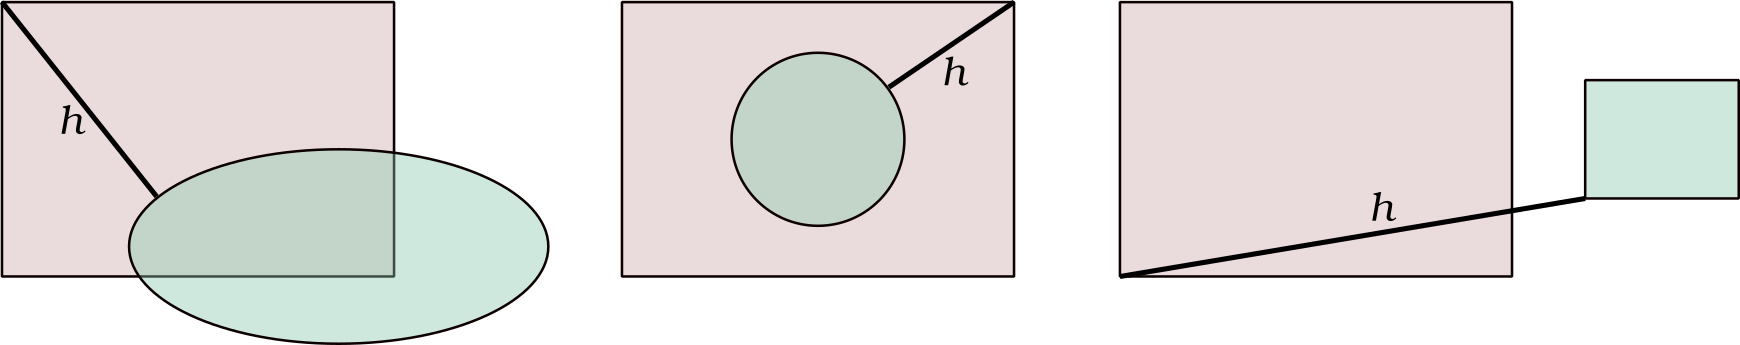
\includegraphics[width=1\textwidth]{images/Hausdorff_distance}}
        \caption[Hausdorffova vzdialenosť]{Hausdorffova vzdialenosť.}
        %id obrazku, pomocou ktoreho sa budeme na obrazok odvolavat
        \label{obr:hausdorff_distance}
    \end{figure}


    Pre nekonečné množiny bodov $M$ a $N$ túto vzdialenosť numericky aproximujeme na konečnej 
    podmnožine bodov $M$ a $N$. Keďže všetky vrcholy meshu ležia so zvolenou presnosťou na ploche, 
    predpokladáme, že body meshu, ktoré sú najvzdialenejšie od plochy sú ťažiská trojuholníkov.
    Ďalej predpokladáme, že najbližší bod z plochy k ťažisku trojuholníka triangulácie
    je kolmý priemet ťažiska na túto plochu.

    Potom diskrétnu numerickú aproximáciu \textit{Hausdorffovej vzdialenosti} definujeme nasledovne.
    \begin{definition}
        Nech $F:\mathbb{R}^3 \to \mathbb{R}$ je funkcia a $S = \{x \in \mathbb{R}^3 \, | \, F(x)=0 \}$ 
        je plocha. Nech $M$ je triangulácia plochy $S$
        a T je množina ťažísk trojuholníkov triangulácie $M$.
        Diskrétnou aproximáciou Hausdorffovej vzdialenosti nazveme vzdialenosť
        \begin{equation}
            h_d = max_{t \in T} \big \{ d(t, t_{proj})\big \},
        \end{equation}
        pričom $t_{proj}$ je priemet bodu $t$ na plochu $S$ v smere vektora $\nabla F(t)$ a
        $d(a, b)$ je euklidovská vzdialenosť v $\mathbb{R}^3$.
    \end{definition}

    Pre zmenšujúcu sa veľkosť hrany očakávame zmenšujúcu sa \textit{diskrétnu Hausdorffovu vzdialenosť}.
    Opäť budeme sledovať aj pomer $h_d : a$. Ak tento pomer pri zmenšovaní dĺžky $a$ klesá, potom 
    \textit{diskrétna Hausdorffova vzdialenosť} klesá rýchlejšie ako zmenšujúca sa dĺžka $a$.

    Kritérium budeme označovať $k_4$.
}
\item{
    \textit{Minimálny a maximálny uhol normál susedných trojuholníkov}

    Keďže $F$ je regulárna plocha, pre zmenšujúcu sa zadanú dĺžku $a$ by sa mal minimálny aj maximálny 
    uhol normál susedných trojuholníkov triangulácie blížiť k nule. Samozrejme, povrchom, ktoré majú 
    v niektorých oblastiach vyššie zakrivenie klesá maximálny uhol normál oveľa pomalšie ako minimálny
    uhol. Toto správanie sa pokúsime sledovať aj na našich modeloch.

    Kritériá budeme označovať $k_5$ (minimálny uhol) a $k_6$ (maximálny uhol).
}
\item{
    \textit{Priemerná vzdialenosť susedných vrcholov od vrchola meshu a smerodajná odchýlka tejto vzdialenosti od priemeru}

    Smerodajná odchýlka hovorí o rozložení hodnôt okolo priemeru. Čím je smerodajná odchýlka menšia, 
    tým bližšie sú hodnoty k priemeru. Naopak, ak je smerodajná odchýlka väčšia, tak sú hodnoty okolo
    priemeru viac rozptýlené.
    
    Majme $N$ hodnôt. Nech $\overline{x}$ označuje aritmetický priemer. 
    Smerodajnú odchýlku môžeme vypočítať podľa nasledujúceho vzorca.

    \begin{equation}
    \label{eq:std}
    \sigma = \sqrt{\frac{1}{N} \sum\limits_{i=1}^{N}(x_i - \overline{x})^2} 
    \end{equation}

    Pre zmenšujúcu sa veľkosť hrany očakávame rovnomerne rozložené vrcholy. Preto očakávame, že 
    priemerná vzdialenosť sa bude blížiť k dĺžke hrany $a$ a smerodajná odchýlka sa bude zmenšovať.
    
    Pre naše modely odmeriame priemer z týchto priemerných vzdialeností (ozn. $p_p$)a takisto priemer 
    zo smerodajných odchýliek (ozn $p_s$). Očakávame, že pomer $p_p : a$ sa bude so zmenšujúcim sa $a$
    blížiť k $1$ a pomer $p_s : a$ sa bude blížiť k $0$.

    Kritériá budeme označovať $k_7$ (priemer) a $k_8$ (smerodajná odchýlka).
}
\end{enumerate}

\section{Konečné plochy}

V tejto kapitole odprezentujeme výsledky meraní kritérií kvality na ôsmych konečných plochách.

\newpage

\begin{enumerate}
\item{
    \textit{Sféra}
    \begin{equation}
    \label{eq:sphere}
    x^2 + y^2 + z^2 - 1 = 0
    \end{equation}

    Na obrázku \ref{obr:sphere} vidíme výslednú trianguláciu sféry danej implicitnou 
    rovnicou \ref{eq:sphere} s piatimi rôznymi dĺžkami strany $a$.
    \begin{enumerate}[a)]
    \item{
        $a=0.9$, $n=64$, $p=34$
    }
    \item{
        $a=0.7$, $n=90$, $p=47$
    }
    \item{
        $a=0.5$, $n=160$, $p=82$
    }
    \item{
        $a=0.3$, $n=408$, $p=206$
    }
    \item{
        $a=0.1$, $n=3246$, $p=1625$
    }
    \end{enumerate}

    \begin{figure}
        \centerline{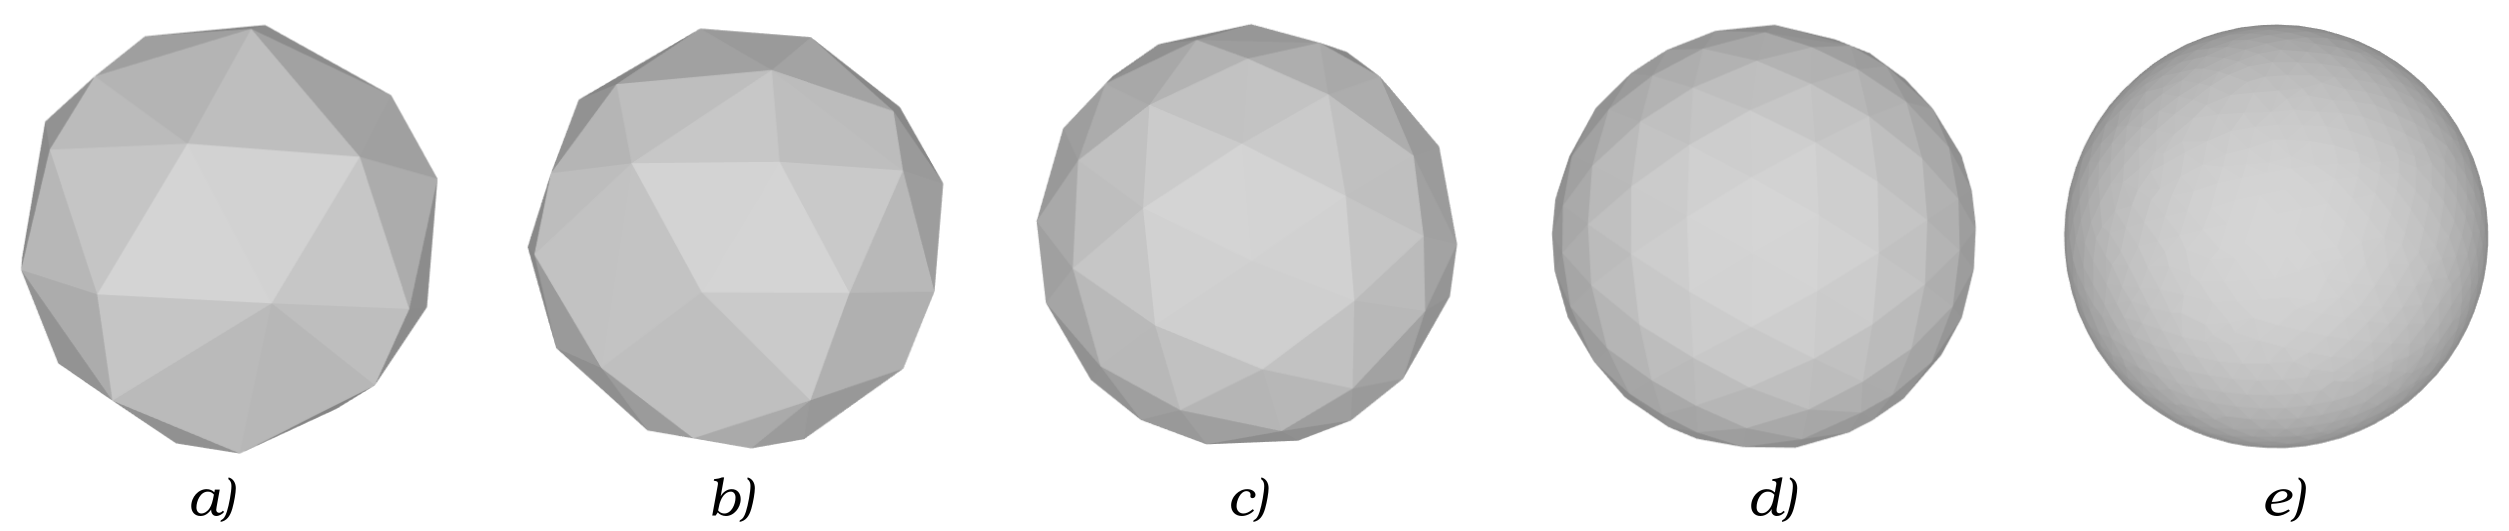
\includegraphics[width=1\textwidth]{images/sphere}}
        \caption[Sféra]{Sféra}
        %id obrazku, pomocou ktoreho sa budeme na obrazok odvolavat
        \label{obr:sphere}
    \end{figure}

    Výsledky merania kritérií kvality môžeme vidieť v tabuľke \ref{tab:sphere}.
    
    \renewcommand*{\MinNumberA}{0.725}%
    \renewcommand*{\MaxNumberA}{0.954}%
    \pgfmathsetmacro{\MidNumberA}{(\MinNumberA+\MaxNumberA)/2}%
    \renewcommand*{\MinNumberB}{0.015}%
    \renewcommand*{\MaxNumberB}{0.085}%
    \pgfmathsetmacro{\MidNumberB}{(\MinNumberB+\MaxNumberB)/2}%
    \renewcommand*{\MinNumberC}{1.210}%
    \renewcommand*{\MaxNumberC}{1.305}%
    \pgfmathsetmacro{\MidNumberC}{(\MinNumberC+\MaxNumberC)/2}%
    \renewcommand*{\MinNumberD}{0.028}%
    \renewcommand*{\MaxNumberD}{0.136}%
    \pgfmathsetmacro{\MidNumberD}{(\MinNumberD+\MaxNumberD)/2}%
    \renewcommand*{\MinNumberE}{0.0}%
    \renewcommand*{\MaxNumberE}{0.051}%
    \pgfmathsetmacro{\MidNumberE}{(\MinNumberE+\MaxNumberE)/2}%
    \renewcommand*{\MinNumberF}{0.120}%
    \renewcommand*{\MaxNumberF}{0.646}%
    \pgfmathsetmacro{\MidNumberF}{(\MinNumberF+\MaxNumberF)/2}%
    \renewcommand*{\MinNumberG}{0.720}%
    \renewcommand*{\MaxNumberG}{0.951}%
    \pgfmathsetmacro{\MidNumberG}{(\MinNumberG+\MaxNumberG)/2}%
    \renewcommand*{\MinNumberH}{0.088}%
    \renewcommand*{\MaxNumberH}{0.112}%
    \pgfmathsetmacro{\MidNumberH}{(\MinNumberH+\MaxNumberH)/2}%


    \begin{table}[ht]
    \label{tab:sphere}
    \caption[Výsledky merania triangulácie sféry]{Výsledky merania}
        \begin{center}
            \begin{tabular}{| c |ABCDEFGH|}
                \hline
                \hline
                \multicolumn{9}{|c|}{Sféra} \\
                \hline
                \hline
                $\hspace{5mm} a \hspace{5mm}$ & $k_1$ & $k_2$ & $k_3$ & $k_4$ & $k_5$ & $k_6$ & $k_7$ & $k_8$ \EndTableHeader\\
                \hline
                \hline
                0.9 & 0.725 & 0.085 & 1.305 & 0.136 & 0.014 & 0.646 & 0.720 & 0.100 \\
                \hline
                0.7 & 0.798 & 0.079 & 1.321 & 0.131 & 0.000 & 0.617 & 0.792 & 0.112 \\
                \hline
                0.5 & 0.847 & 0.062 & 1.253 & 0.104 & 0.051 & 0.472 & 0.843 & 0.097 \\
                \hline
                0.3 & 0.895 & 0.041 & 1.274 & 0.074 & 0.000 & 0.291 & 0.892 & 0.103 \\
                \hline
                0.1 & 0.954 & 0.015 & 1.210 & 0.028 & 0.000 & 0.120 & 0.951 & 0.088 \\
                \hline
                \hline
            \end{tabular}
        \end{center}
    \end{table}

}

\newpage

\item{
    \textit{Elipsoid}
    \begin{equation}
    \label{eq:ellipsoid}
        \bigg ( \frac{x-1}{2} \bigg )^2 + \bigg (\frac{y-1}{3} \bigg )^2 + (z - 1)^2 - 1 = 0
    \end{equation}

    Na obrázku \ref{obr:ellipsoid} vidíme výslednú trianguláciu elipsoidu daného implicitnou 
    rovnicou \ref{eq:ellipsoid} s piatimi rôznymi dĺžkami strany $a$.
    \begin{enumerate}[a)]
    \item{
        $a=0.9$, $n=214$, $p=109$
    }
    \item{
        $a=0.7$, $n=332$, $p=168$
    }
    \item{
        $a=0.5$, $n=574$, $p=289$
    }
    \item{
        $a=0.3$, $n=1460$, $p=732$
    }
    \item{
        $a=0.15$, $n=5476$, $p=2740$
    }
    \end{enumerate}

    \begin{figure}
        \centerline{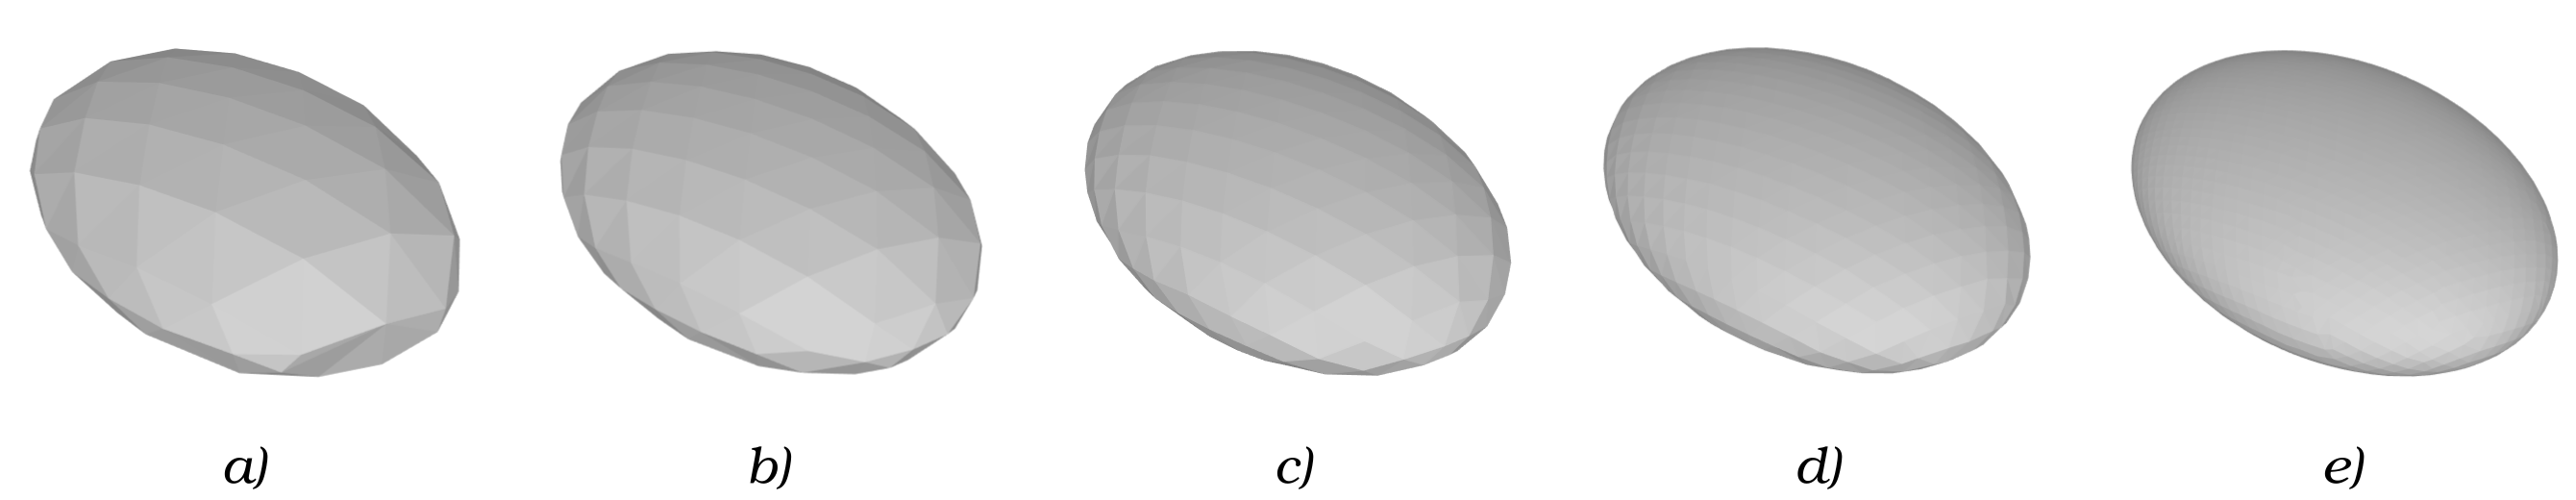
\includegraphics[width=1\textwidth]{images/ellipsoid}}
        \caption[Elipsoid]{Elipsoid}
        %id obrazku, pomocou ktoreho sa budeme na obrazok odvolavat
        \label{obr:ellipsoid}
    \end{figure}

    Výsledky merania kritérií kvality môžeme vidieť v tabuľke \ref{tab:ellipsoid}.

    \renewcommand*{\MinNumberA}{0.802}%
    \renewcommand*{\MaxNumberA}{0.962}%
    \pgfmathsetmacro{\MidNumberA}{(\MinNumberA+\MaxNumberA)/2}%
    \renewcommand*{\MinNumberB}{0.013}%
    \renewcommand*{\MaxNumberB}{0.049}%
    \pgfmathsetmacro{\MidNumberB}{(\MinNumberB+\MaxNumberB)/2}%
    \renewcommand*{\MinNumberC}{1.142}%
    \renewcommand*{\MaxNumberC}{1.356}%
    \pgfmathsetmacro{\MidNumberC}{(\MinNumberC+\MaxNumberC)/2}%
    \renewcommand*{\MinNumberD}{0.057}%
    \renewcommand*{\MaxNumberD}{0.192}%
    \pgfmathsetmacro{\MidNumberD}{(\MinNumberD+\MaxNumberD)/2}%
    \renewcommand*{\MinNumberE}{0.0}%
    \renewcommand*{\MaxNumberE}{0.00073}%
    \pgfmathsetmacro{\MidNumberE}{(\MinNumberE+\MaxNumberE)/2}%
    \renewcommand*{\MinNumberF}{0.338}%
    \renewcommand*{\MaxNumberF}{1.122}%
    \pgfmathsetmacro{\MidNumberF}{(\MinNumberF+\MaxNumberF)/2}%
    \renewcommand*{\MinNumberG}{0.796}%
    \renewcommand*{\MaxNumberG}{0.961}%
    \pgfmathsetmacro{\MidNumberG}{(\MinNumberG+\MaxNumberG)/2}%
    \renewcommand*{\MinNumberH}{0.061}%
    \renewcommand*{\MaxNumberH}{0.116}%
    \pgfmathsetmacro{\MidNumberH}{(\MinNumberH+\MaxNumberH)/2}%

    \begin{table}[ht]
    \label{tab:ellipsoid}
    \caption[Výsledky merania triangulácie elipsoidu]{Výsledky merania}
        \begin{center}
            \begin{tabular}{|c|A B C D E F G H|}
                \hline
                \hline
                \multicolumn{9}{|c|}{Elipsoid} \\
                \hline
                \hline
                $\hspace{5mm} a \hspace{5mm}$ & $k_1$ & $k_2$ & $k_3$ & $k_4$ & $k_5$ & $k_6$ & $k_7$ & $k_8$ \EndTableHeader\\
                \hline
                \hline
                0.9 & 0.802 & 0.049 & 1.356 & 0.192 & 
                0.00073 & 1.220 & 0.796 & 0.116 \\
                \hline
                0.7 & 0.828 & 0.041 & 1.271 & 0.084 & 
                0.00017 & 0.888 & 0.823 & 0.098\\
                \hline
                0.5 & 0.881 & 0.035 & 1.204 & 0.084 & 
                0.00039 & 0.745 & 0.881 & 0.083\\
                \hline
                0.3 & 0.928 & 0.024 & 1.169 & 0.093 & 
                0.00003 & 0.597 & 0.928 & 0.067\\
                \hline
                0.15 & 0.962 & 0.013 & 1.142 & 0.057 & 
                0.00000 & 0.338 & 0.961 & 0.061\\
                \hline
                \hline
            \end{tabular}
        \end{center}
    \end{table}
}


\newpage

\item{
    \textit{Zaoblená kocka}
    \begin{equation}
    \label{eq:cubed_sphere}
        x^4+y^4+z^4-1 = 0
    \end{equation}

    Na obrázku \ref{obr:cubed_sphere} vidíme výslednú trianguláciu zaoblenej kocky danej implicitnou 
    rovnicou \ref{eq:cubed_sphere} s piatimi rôznymi dĺžkami strany $a$.
    \begin{enumerate}[a)]
    \item{
        $a=2$, $n=30$, $p=17$
    }
    \item{
        $a=1$, $n=68$, $p=36$
    }
    \item{
        $a=0.5$, $n=216$, $p=110$
    }
    \item{
        $a=0.25$, $n=748$, $p=376$
    }
    \item{
        $a=0.15$, $n=2034$, $p=1018$
    }
    \end{enumerate}

    \begin{figure}
        \centerline{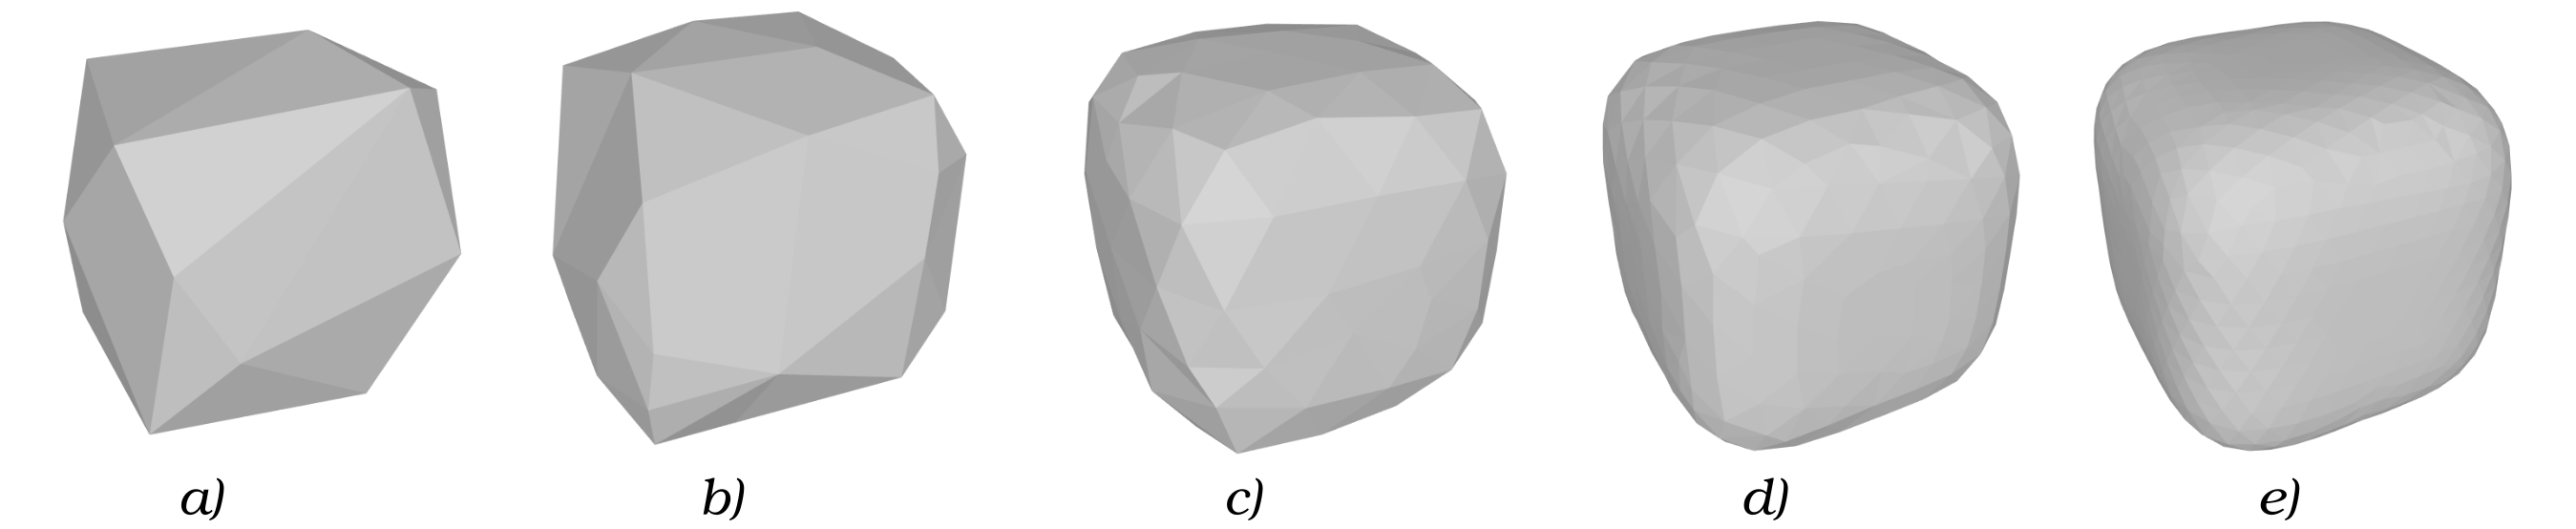
\includegraphics[width=1\textwidth]{images/cubed_sphere}}
        \caption[Zaoblená kocka]{Zaoblená kocka}
        %id obrazku, pomocou ktoreho sa budeme na obrazok odvolavat
        \label{obr:cubed_sphere}
    \end{figure}

    Výsledky merania kritérií kvality môžeme vidieť v tabuľke \ref{tab:cubed_sphere}.

    \renewcommand*{\MinNumberA}{0.555}%
    \renewcommand*{\MaxNumberA}{0.949}%
    \pgfmathsetmacro{\MidNumberA}{(\MinNumberA+\MaxNumberA)/2}%
    \renewcommand*{\MinNumberB}{0.020}%
    \renewcommand*{\MaxNumberB}{0.077}%
    \pgfmathsetmacro{\MidNumberB}{(\MinNumberB+\MaxNumberB)/2}%
    \renewcommand*{\MinNumberC}{1.189}%
    \renewcommand*{\MaxNumberC}{1.681}%
    \pgfmathsetmacro{\MidNumberC}{(\MinNumberC+\MaxNumberC)/2}%
    \renewcommand*{\MinNumberD}{0.069}%
    \renewcommand*{\MaxNumberD}{0.244}%
    \pgfmathsetmacro{\MidNumberD}{(\MinNumberD+\MaxNumberD)/2}%
    \renewcommand*{\MinNumberE}{0.00004}%
    \renewcommand*{\MaxNumberE}{0.00524}%
    \pgfmathsetmacro{\MidNumberE}{(\MinNumberE+\MaxNumberE)/2}%
    \renewcommand*{\MinNumberF}{0.348}%
    \renewcommand*{\MaxNumberF}{1.128}%
    \pgfmathsetmacro{\MidNumberF}{(\MinNumberF+\MaxNumberF)/2}%
    \renewcommand*{\MinNumberG}{0.548}%
    \renewcommand*{\MaxNumberG}{0.947}%
    \pgfmathsetmacro{\MidNumberG}{(\MinNumberG+\MaxNumberG)/2}%
    \renewcommand*{\MinNumberH}{0.079}%
    \renewcommand*{\MaxNumberH}{0.152}%
    \pgfmathsetmacro{\MidNumberH}{(\MinNumberH+\MaxNumberH)/2}%
    
     \begin{table}[ht]
     \label{tab:cubed_sphere}
     \caption[Výsledky merania triangulácie zaoblenej kocky]{Výsledky merania}
        \begin{center}
            \begin{tabular}{|c|A B C D E F G H|}
                \hline
                \hline
                \multicolumn{9}{|c|}{Zaoblená kocka} \\
                \hline
                \hline
                $\hspace{5mm} a \hspace{5mm}$ & $k_1$ & $k_2$ & $k_3$ & $k_4$ & $k_5$ & $k_6$ & $k_7$ & $k_8$ \EndTableHeader\\
                \hline
                \hline
                2 & 0.555 & 0.066 & 1.681 & 0.143 & 0.00482 & 1.228 & 0.548 & 0.136\\
                \hline
                1 & 0.750 & 0.077 & 1.454 & 0.244 & 0.00524 & 1.062 & 0.738 & 0.152\\
                \hline
                0.5 & 0.865 & 0.051 & 1.286 & 0.173 & 0.00040 & 0.837 & 0.861 & 0.111\\
                \hline
                0.25 & 0.935 & 0.031 & 1.189 & 0.099 & 0.00026 & 0.591 & 0.932 & 0.080\\
                \hline
                0.15 & 0.949 & 0.020 & 1.189 & 0.069 & 0.00004 & 0.348 & 0.947 & 0.079\\
                \hline
                \hline
            \end{tabular}
        \end{center}
    \end{table}
}

\newpage

\item{
    \textit{Torus}
    \begin{equation}
    \label{eq:torus}
        (x^2+y^2+z^2+1375)^2-6400(x^2+y^2) = 0
    \end{equation}

    Na obrázku \ref{obr:torus} vidíme výslednú trianguláciu torusu daného implicitnou 
    rovnicou \ref{eq:torus} s piatimi rôznymi dĺžkami strany $a$.
    \begin{enumerate}[a)]
    \item{
        $a=15$, $n=334$, $p=167$
    }
    \item{
        $a=12$, $n=494$, $p=247$
    }
    \item{
        $a=9$, $n=818$, $p=409$
    }
    \item{
        $a=6$, $n=1720$, $p=860$
    }
    \item{
        $a=3$, $n=6596$, $p=3297$
    }
    \end{enumerate}

    \begin{figure}
        \centerline{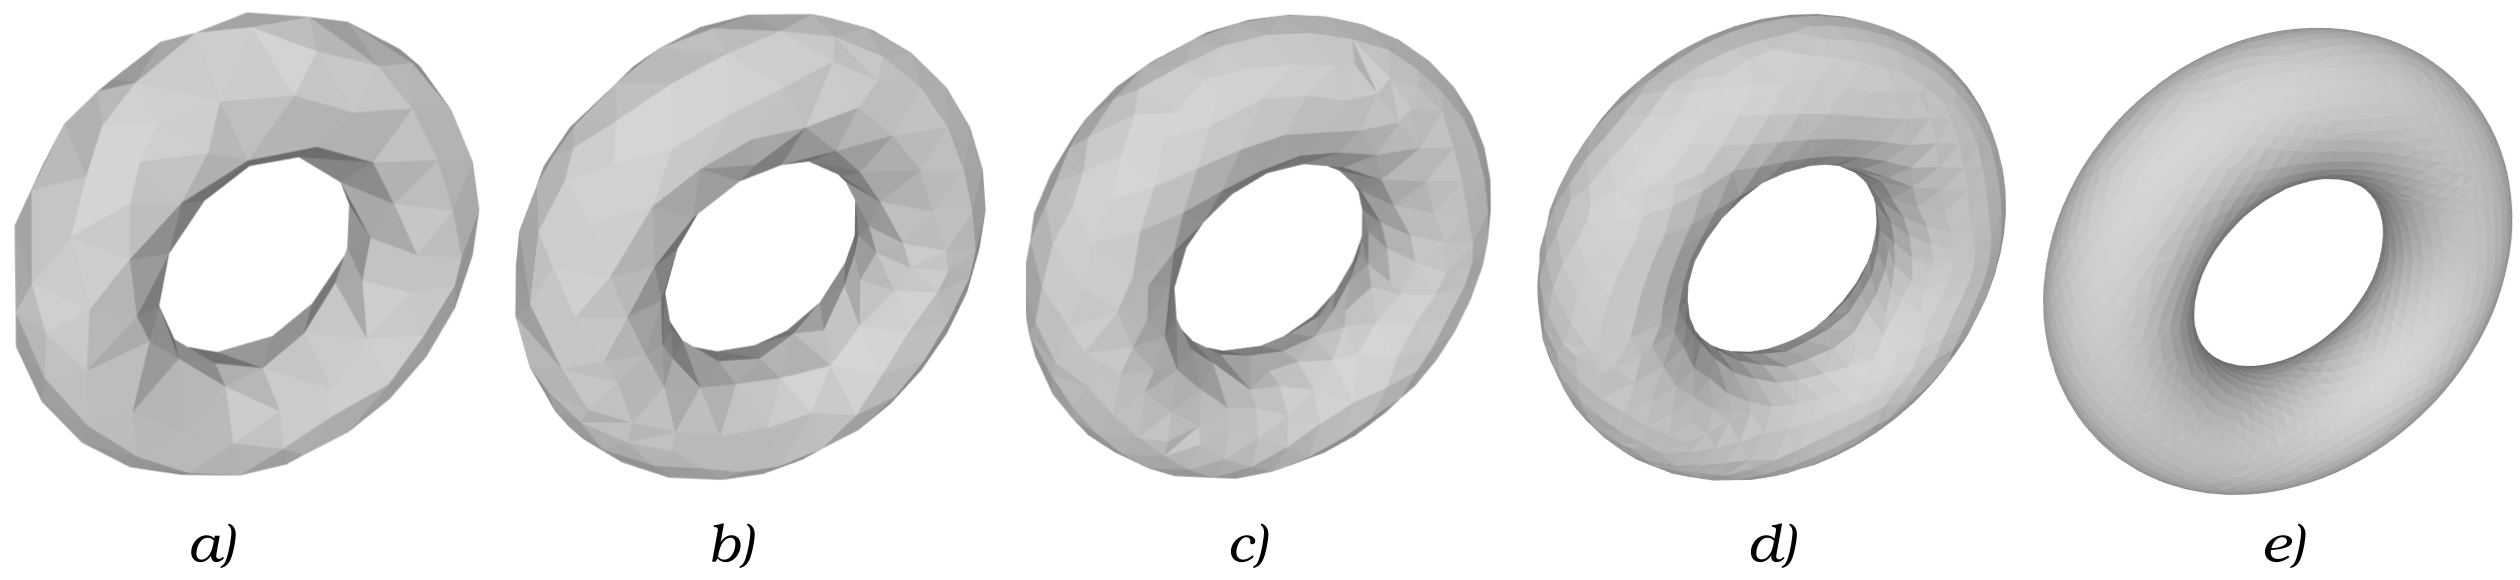
\includegraphics[width=1\textwidth]{images/torus}}
        \caption[Torus]{Torus}
        %id obrazku, pomocou ktoreho sa budeme na obrazok odvolavat
        \label{obr:torus}
    \end{figure}

    Výsledky merania kritérií kvality môžeme vidieť v tabuľke \ref{tab:torus}.

     
    \renewcommand*{\MinNumberA}{0.856}%
    \renewcommand*{\MaxNumberA}{0.968}%
    \pgfmathsetmacro{\MidNumberA}{(\MinNumberA+\MaxNumberA)/2}%
    \renewcommand*{\MinNumberB}{0.016}%
    \renewcommand*{\MaxNumberB}{0.060}%
    \pgfmathsetmacro{\MidNumberB}{(\MinNumberB+\MaxNumberB)/2}%
    \renewcommand*{\MinNumberC}{1.197}%
    \renewcommand*{\MaxNumberC}{1.331}%
    \pgfmathsetmacro{\MidNumberC}{(\MinNumberC+\MaxNumberC)/2}%
    \renewcommand*{\MinNumberD}{0.052}%
    \renewcommand*{\MaxNumberD}{0.188}%
    \pgfmathsetmacro{\MidNumberD}{(\MinNumberD+\MaxNumberD)/2}%
    \renewcommand*{\MinNumberE}{0.00000}%
    \renewcommand*{\MaxNumberE}{0.00067}%
    \pgfmathsetmacro{\MidNumberE}{(\MinNumberE+\MaxNumberE)/2}%
    \renewcommand*{\MinNumberF}{0.467}%
    \renewcommand*{\MaxNumberF}{0.974}%
    \pgfmathsetmacro{\MidNumberF}{(\MinNumberF+\MaxNumberF)/2}%
    \renewcommand*{\MinNumberG}{0.851}%
    \renewcommand*{\MaxNumberG}{0.966}%
    \pgfmathsetmacro{\MidNumberG}{(\MinNumberG+\MaxNumberG)/2}%
    \renewcommand*{\MinNumberH}{0.083}%
    \renewcommand*{\MaxNumberH}{0.117}%
    \pgfmathsetmacro{\MidNumberH}{(\MinNumberH+\MaxNumberH)/2}%

  
     \begin{table}[ht]
     \label{tab:torus}
     \caption[Výsledky merania triangulácie torusu]{Výsledky merania}
        \begin{center}
            \begin{tabular}{|c|A B C D E F G H|}
                \hline
                \hline
                \multicolumn{9}{|c|}{Torus} \\
                \hline
                \hline
                $\hspace{5mm} a \hspace{5mm}$ & $k_1$ & $k_2$ & $k_3$ & $k_4$ & $k_5$ & $k_6$ & $k_7$ & $k_8$ \EndTableHeader\\
                \hline
                \hline
                15 & 0.856 & 0.060 & 1.324 & 0.188 & 0.00000 & 0.974 & 0.851 & 0.116\\
                \hline
                12 & 0.882 & 0.051 & 1.331 & 0.151 & 0.00067 & 0.823 & 0.878 & 0.117\\
                \hline
                9 & 0.916 & 0.042 & 1.284 & 0.097 & 0.00013 & 0.671 & 0.912 & 0.109\\
                \hline
                6 & 0.946 & 0.030 & 1.227 & 0.078 & 0.00001 & 0.467 & 0.944 & 0.094\\
                \hline
                3 & 0.968 & 0.016 & 1.197 & 0.052 & 0.00002 & 0.868 & 0.966 & 0.083\\
                \hline
                \hline
            \end{tabular}
        \end{center}
    \end{table}

}

\newpage

\item{
    \textit{Genus}
    \begin{equation}
    \label{eq:genus}
        (x^2+y^2+z^2+1375)^2-6400(x^2+y^2) = 0
    \end{equation}

    Na obrázku \ref{obr:genus} vidíme výslednú trianguláciu torusu daného implicitnou 
    rovnicou \ref{eq:genus} s piatimi rôznymi dĺžkami strany $a$.
    \begin{enumerate}[a)]
    \item{
        $a=15$, $n=334$, $p=$
    }
    \item{
        $a=12$, $n=494$, $p=$
    }
    \item{
        $a=9$, $n=818$, $p=$
    }
    \item{
        $a=6$, $n=1720$, $p=$
    }
    \item{
        $a=3$, $n=6596$, $p=$
    }
    \end{enumerate}

    \begin{figure}
        \centerline{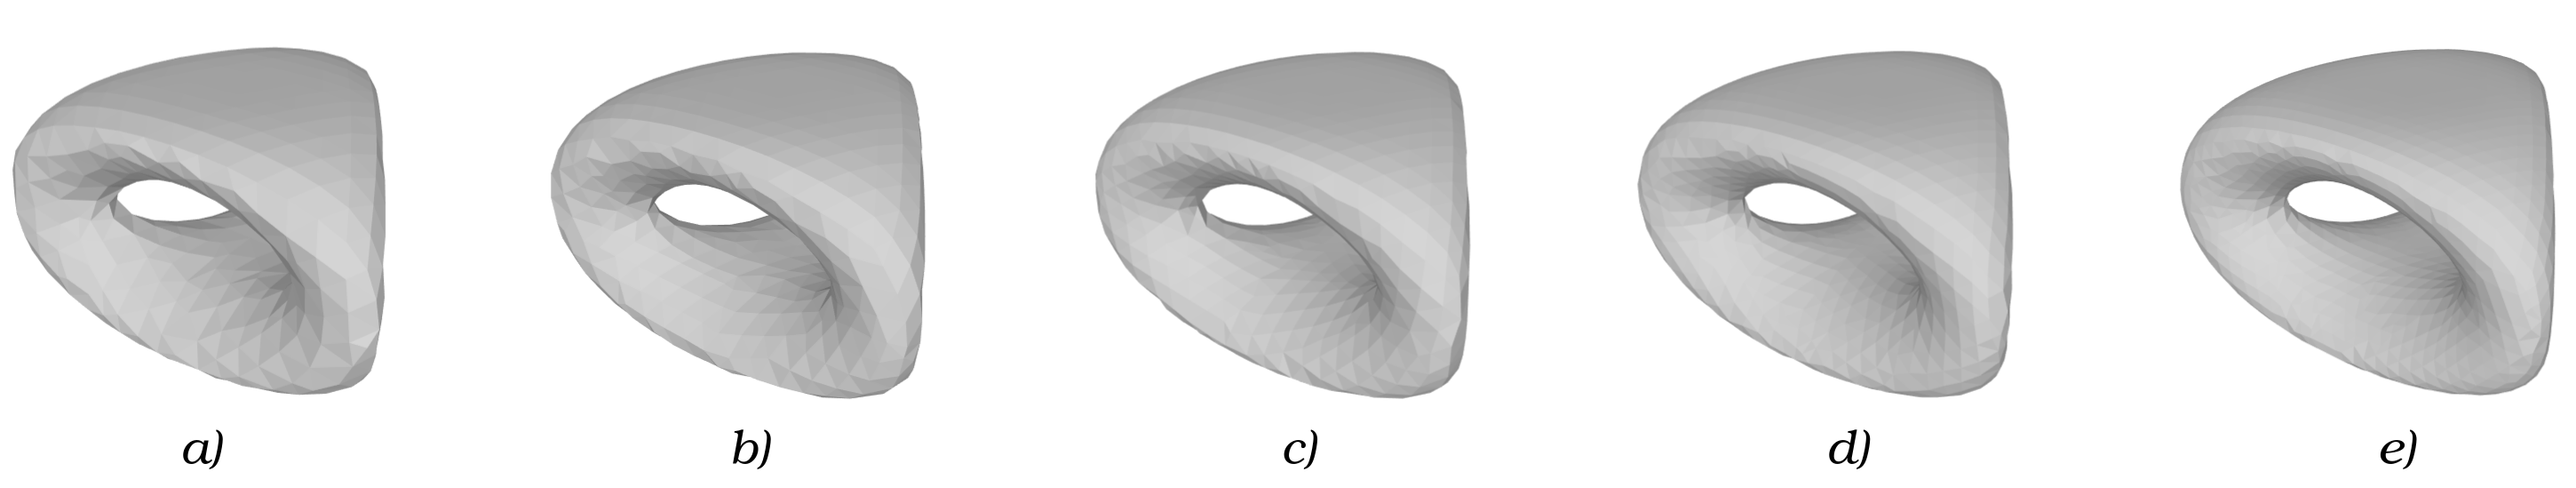
\includegraphics[width=1\textwidth]{images/genus}}
        \caption[Genus]{Genus}
        %id obrazku, pomocou ktoreho sa budeme na obrazok odvolavat
        \label{obr:genus}
    \end{figure}

    Výsledky merania kritérií kvality môžeme vidieť v tabuľke \ref{tab:genus}.

    \begin{table}[ht]
     \label{tab:genus}
     \caption[Výsledky merania triangulácie genusu]{Výsledky merania}
        \begin{center}
            \begin{tabular}{|c|A B C D E F G H|}
                \hline
                \multicolumn{9}{|c|}{Genus} \\
                \hline
                $\hspace{8mm} a \hspace{8mm}$ & $k_1$ & $k_2$ & $k_3$ & $k_4$ & $k_5$ & $k_6$ & $k_7$ & $k_8$ \EndTableHeader\\
                \hline
                0.225 & 0.808 & 0.029 & 0.912 & 0.9 & 0.629 & 0.049 & 0.802 & 0.802\\
                \hline
                0.2 & 0.819 & 0.027 & 0.918 & 0.9 & 0.629 & 0.049 & 0.802 & 0.802\\
                \hline
                0.175 & 0.845 & 0.024 & 0.931 & 0.9 & 0.629 & 0.049 & 0.802 & 0.802\\
                \hline
                0.15 & 0.858 & 0.021 & 0.937 & 0.9 & 0.629 & 0.049 & 0.802 & 0.802\\
                \hline
                0.125 & 0.892 & 0.018 & 0.954 & 0.9 & 0.629 & 0.049 & 0.802 & 0.802\\
                \hline
                \hline
            \end{tabular}
        \end{center}
    \end{table}

}
\newpage

\item{
    \textit{Tetrahedron}
    \begin{equation}
    \label{eq:tetrahedron}
        (x^2+y^2+z^2+1375)^2-6400(x^2+y^2) = 0
    \end{equation}

    Na obrázku \ref{obr:tetrahedron} vidíme výslednú trianguláciu torusu daného implicitnou 
    rovnicou \ref{eq:tetrahedron} s piatimi rôznymi dĺžkami strany $a$.
    \begin{enumerate}[a)]
    \item{
        $a=15$, $n=334$, $p=$
    }
    \item{
        $a=12$, $n=494$, $p=$
    }
    \item{
        $a=9$, $n=818$, $p=$
    }
    \item{
        $a=6$, $n=1720$, $p=$
    }
    \item{
        $a=3$, $n=6596$, $p=$
    }
    \end{enumerate}

    \begin{figure}
        \centerline{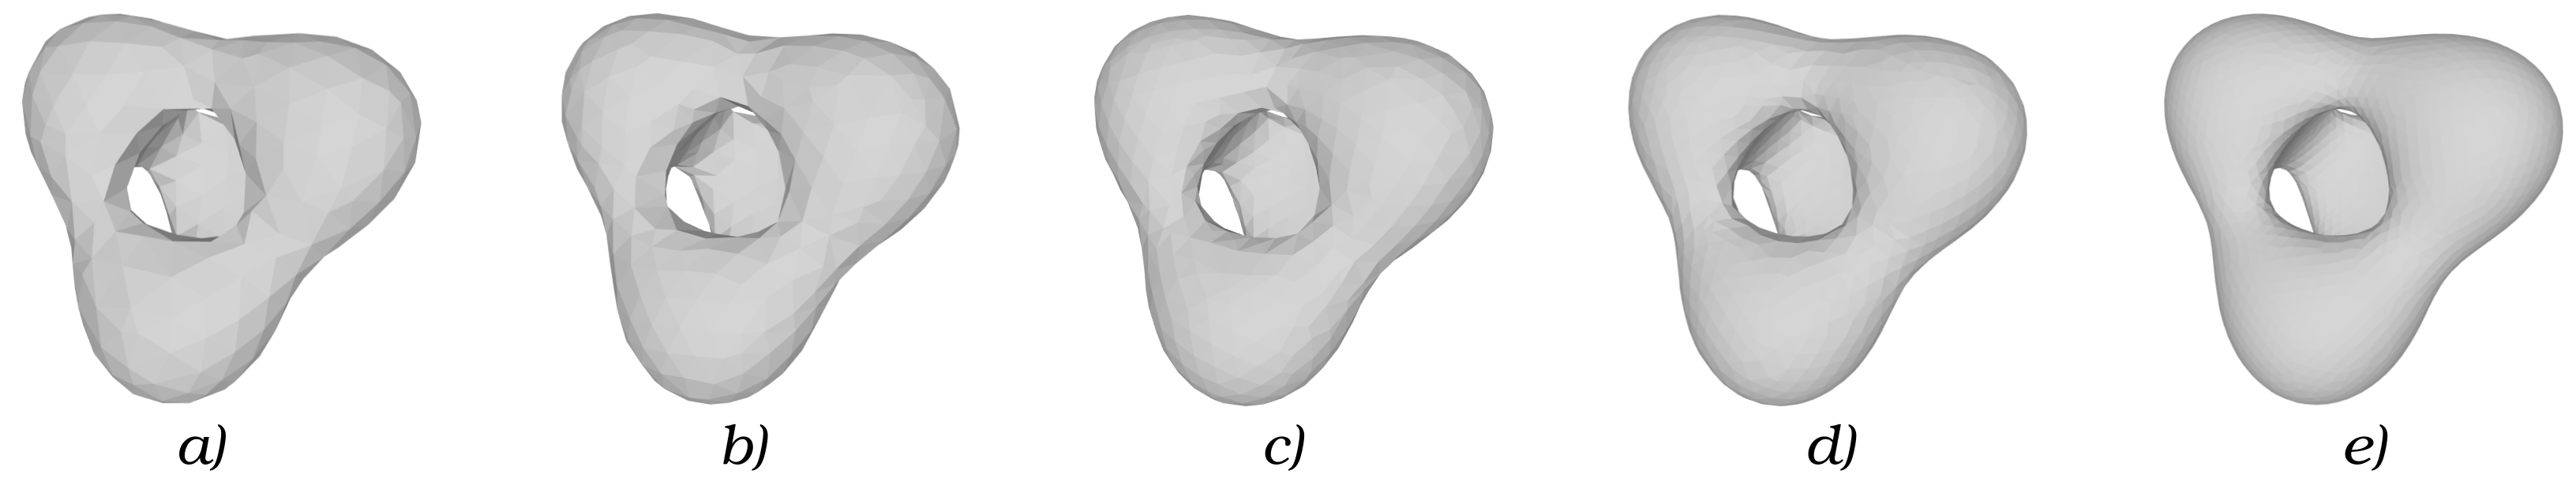
\includegraphics[width=1\textwidth]{images/tetrahedron}}
        \caption[Tetrahedron]{Tetrahedron}
        %id obrazku, pomocou ktoreho sa budeme na obrazok odvolavat
        \label{obr:tetrahedron}
    \end{figure}

    Výsledky merania kritérií kvality môžeme vidieť v tabuľke \ref{tab:tetrahedron}.

    \begin{table}[ht]
     \label{tab:tetrahedron}
     \caption[Výsledky merania triangulácie tetrahedronu]{Výsledky merania}
        \begin{center}
            \begin{tabular}{|c|A B C D E F G H|}
                \hline
                \multicolumn{9}{|c|}{Tetrahedron} \\
                \hline
                $\hspace{8mm} a \hspace{8mm}$ & $k_1$ & $k_2$ & $k_3$ & $k_4$ & $k_5$ & $k_6$ & $k_7$ & $k_8$ \EndTableHeader\\
                \hline
                0.225 & 0.808 & 0.029 & 0.912 & 0.9 & 0.629 & 0.049 & 0.802 & 0.802\\
                \hline
                0.2 & 0.819 & 0.027 & 0.918 & 0.9 & 0.629 & 0.049 & 0.802 & 0.802\\
                \hline
                0.175 & 0.845 & 0.024 & 0.931 & 0.9 & 0.629 & 0.049 & 0.802 & 0.802\\
                \hline
                0.15 & 0.858 & 0.021 & 0.937 & 0.9 & 0.629 & 0.049 & 0.802 & 0.802\\
                \hline
                0.125 & 0.892 & 0.018 & 0.954 & 0.9 & 0.629 & 0.049 & 0.802 & 0.802\\
                \hline
                \hline
            \end{tabular}
        \end{center}
    \end{table}

}
\newpage
\item{
    \textit{Plocha konštantného súčinu vzdialeností od štvorice bodov}
    \begin{equation}
    \label{eq:blobby}
        (x^2+y^2+z^2+1375)^2-6400(x^2+y^2) = 0
    \end{equation}

    Na obrázku \ref{obr:blobby} vidíme výslednú trianguláciu plochy danej implicitnou 
    rovnicou \ref{eq:blobby} s piatimi rôznymi dĺžkami strany $a$.
    \begin{enumerate}[a)]
    \item{
        $a=15$, $n=334$, $p=$
    }
    \item{
        $a=12$, $n=494$, $p=$
    }
    \item{
        $a=9$, $n=818$, $p=$
    }
    \item{
        $a=6$, $n=1720$, $p=$
    }
    \item{
        $a=3$, $n=6596$, $p=$
    }
    \end{enumerate}

    \begin{figure}
        \centerline{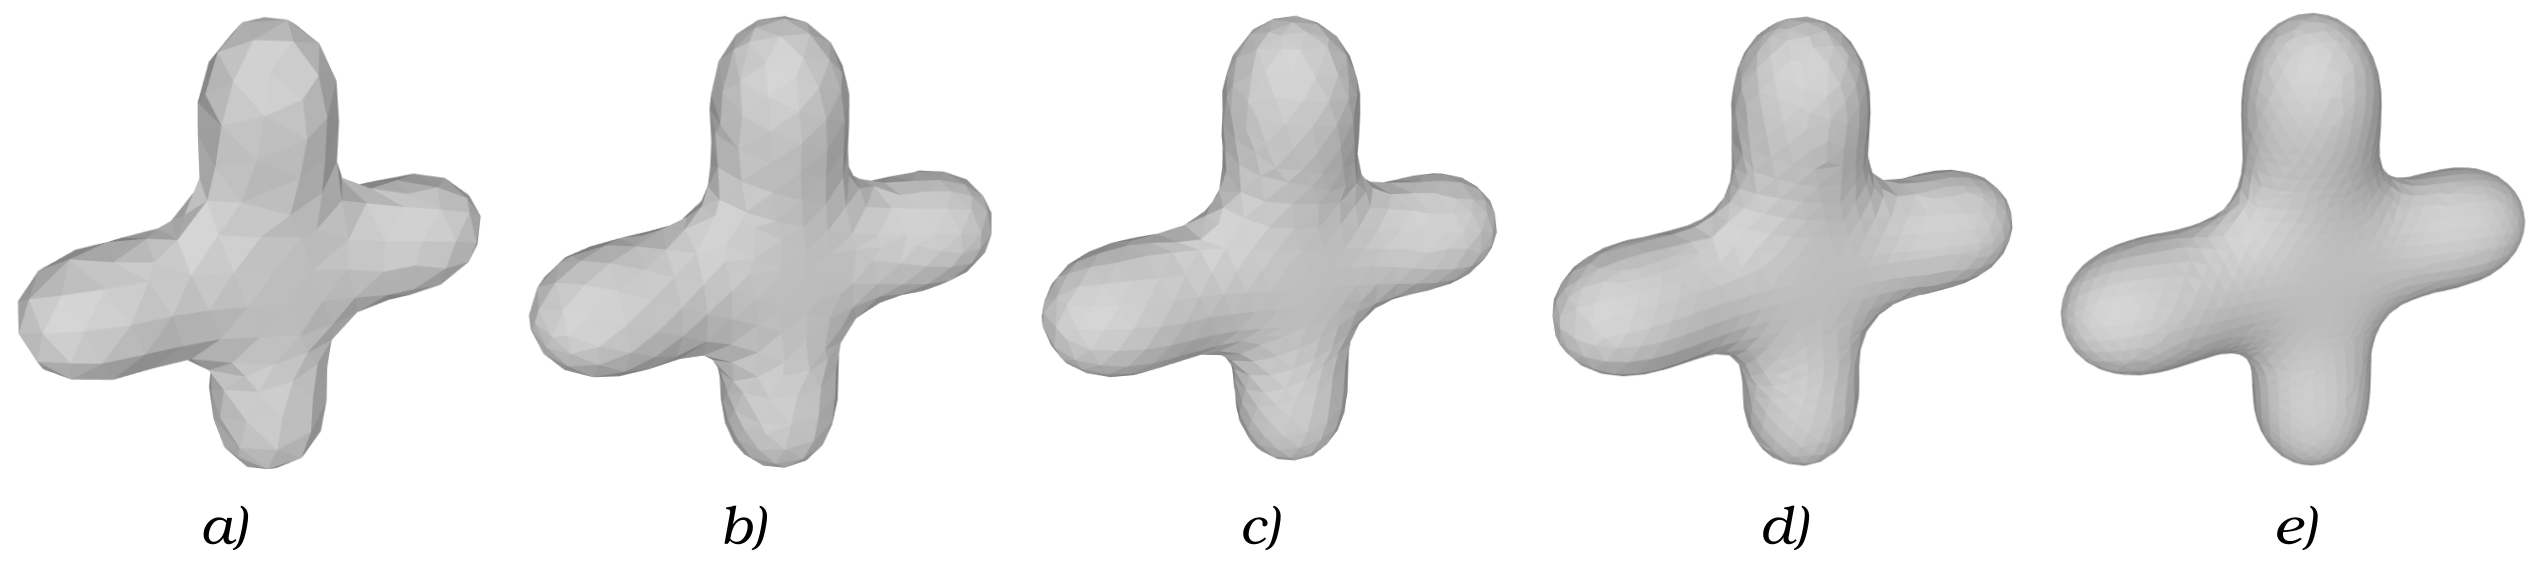
\includegraphics[width=1\textwidth]{images/blobby}}
        \caption[Plocha konštantného súčinu vzdialeností od štvorice bodov]
        {Plocha konštantného súčinu vzdialeností od štvorice bodov}
        %id obrazku, pomocou ktoreho sa budeme na obrazok odvolavat
        \label{obr:blobby}
    \end{figure}

    Výsledky merania kritérií kvality môžeme vidieť v tabuľke \ref{tab:blobby}.

    \begin{table}[ht]
     \label{tab:blobby}
     \caption[Výsledky merania triangulácie plochy konštantného súčinu vzdialeností od štvorice bodov]{Výsledky merania}
        \begin{center}
            \begin{tabular}{|c|A B C D E F G H|}
                \hline
                \multicolumn{9}{|c|}{Plocha konštantného súčinu vzdialeností od štvorice bodov} \\
                \hline
                $\hspace{8mm} a \hspace{8mm}$ & $k_1$ & $k_2$ & $k_3$ & $k_4$ & $k_5$ & $k_6$ & $k_7$ & $k_8$ \EndTableHeader\\
                \hline
                0.225 & 0.808 & 0.029 & 0.912 & 0.9 & 0.629 & 0.049 & 0.802 & 0.802\\
                \hline
                0.2 & 0.819 & 0.027 & 0.918 & 0.9 & 0.629 & 0.049 & 0.802 & 0.802\\
                \hline
                0.175 & 0.845 & 0.024 & 0.931 & 0.9 & 0.629 & 0.049 & 0.802 & 0.802\\
                \hline
                0.15 & 0.858 & 0.021 & 0.937 & 0.9 & 0.629 & 0.049 & 0.802 & 0.802\\
                \hline
                0.125 & 0.892 & 0.018 & 0.954 & 0.9 & 0.629 & 0.049 & 0.802 & 0.802\\
                \hline
                \hline
            \end{tabular}
        \end{center}
    \end{table}

}

\newpage
\item{
    \textit{Plocha \textit{tanglecube}}
    \begin{equation}
    \label{eq:joined_spheres}
        (x^2+y^2+z^2+1375)^2-6400(x^2+y^2) = 0
    \end{equation}

    Na obrázku \ref{obr:joined_spheres} vidíme výslednú trianguláciu plochy \textit{tanglecube} 
    danej implicitnou rovnicou \ref{eq:joined_spheres} s piatimi rôznymi dĺžkami strany $a$.
    \begin{enumerate}[a)]
    \item{
        $a=15$, $n=334$, $p=$
    }
    \item{
        $a=12$, $n=494$, $p=$
    }
    \item{
        $a=9$, $n=818$, $p=$
    }
    \item{
        $a=6$, $n=1720$, $p=$
    }
    \item{
        $a=3$, $n=6596$, $p=$
    }
    \end{enumerate}

    \begin{figure}
        \centerline{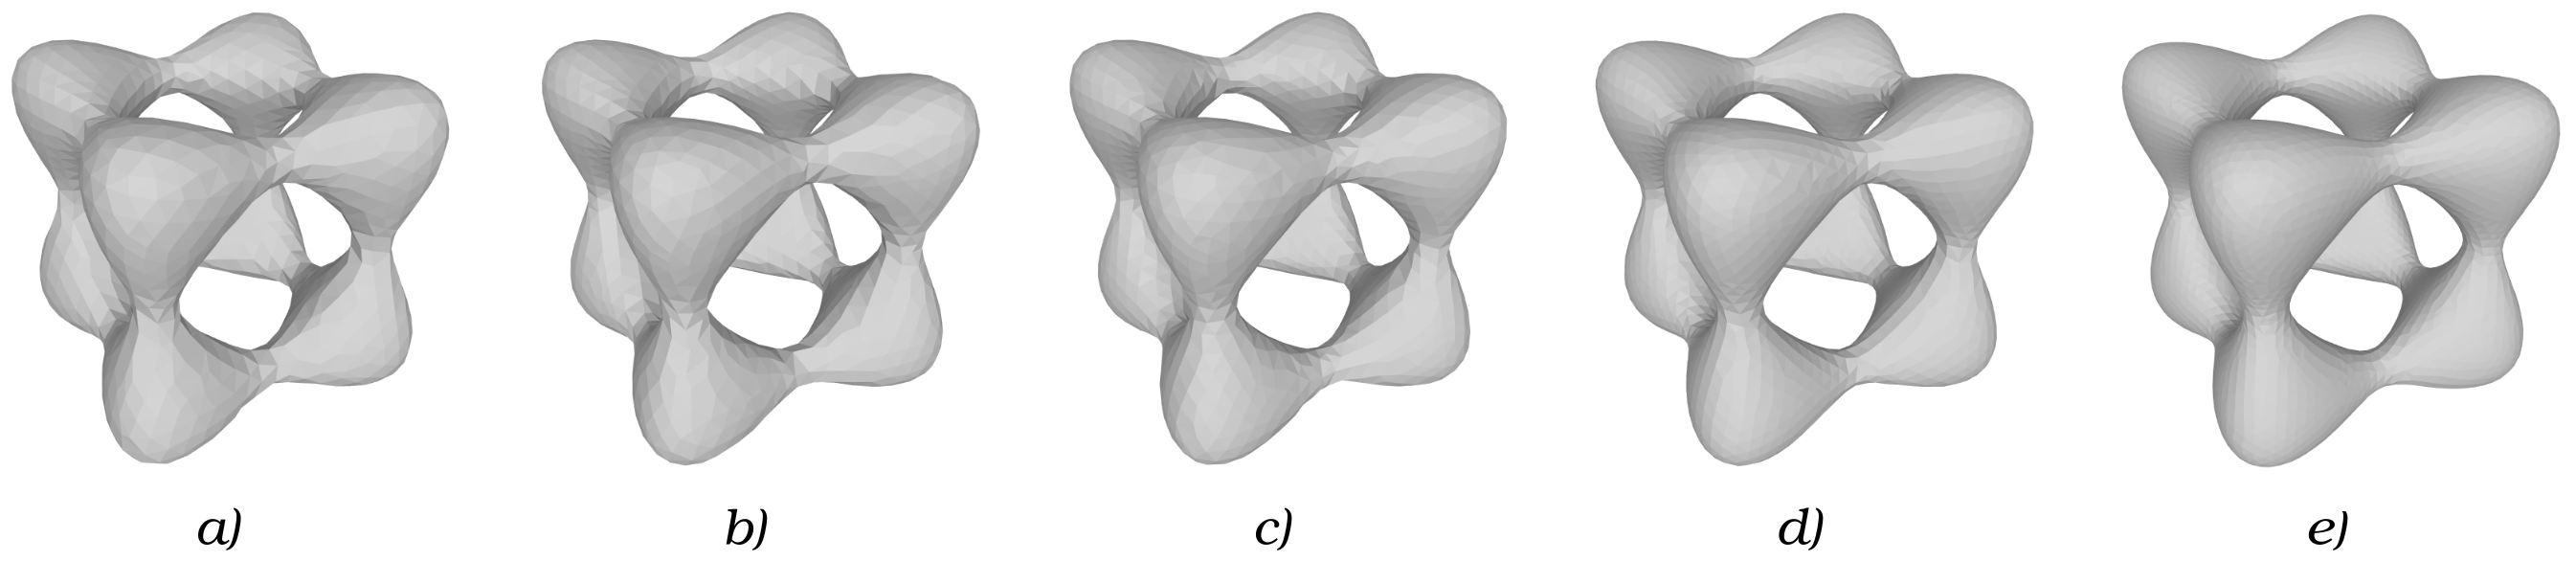
\includegraphics[width=1\textwidth]{images/joined_spheres}}
        \caption[Plocha \textit{tanglecube}]{Plocha \textit{tanglecube}}
        %id obrazku, pomocou ktoreho sa budeme na obrazok odvolavat
        \label{obr:joined_spheres}
    \end{figure}

    Výsledky merania kritérií kvality môžeme vidieť v tabuľke \ref{tab:joined_spheres}.

    \begin{table}[ht]
     \label{tab:joined_spheres}
     \caption[Výsledky merania triangulácie plochy\textit{tanglecube}]{Výsledky merania}
        \begin{center}
            \begin{tabular}{|c|A B C D E F G H|}
                \hline
                \multicolumn{9}{|c|}{Plocha \textit{tanglecube}} \\
                \hline
                $\hspace{8mm} a \hspace{8mm}$ & $k_1$ & $k_2$ & $k_3$ & $k_4$ & $k_5$ & $k_6$ & $k_7$ & $k_8$ \EndTableHeader\\
                \hline
                0.225 & 0.808 & 0.029 & 0.912 & 0.9 & 0.629 & 0.049 & 0.802 & 0.802\\
                \hline
                0.2 & 0.819 & 0.027 & 0.918 & 0.9 & 0.629 & 0.049 & 0.802 & 0.802\\
                \hline
                0.175 & 0.845 & 0.024 & 0.931 & 0.9 & 0.629 & 0.049 & 0.802 & 0.802\\
                \hline
                0.15 & 0.858 & 0.021 & 0.937 & 0.9 & 0.629 & 0.049 & 0.802 & 0.802\\
                \hline
                0.125 & 0.892 & 0.018 & 0.954 & 0.9 & 0.629 & 0.049 & 0.802 & 0.802\\
                \hline
                \hline
            \end{tabular}
        \end{center}
    \end{table}

}
     

\end{enumerate}

\newpage
\subsection{Pozorovania}
Po skončení algoritmu pre dostatočne malú veľkosť hrany vznikajú korektné triangulácie,
bez prekrývania trojuholníkov a taktiež bez dier. Aj napriek tomu, že po teoretickej stránke
môžu vznikať triangulácie aj s dierami či prekrytými trojuholníkmi, 
v našich pozorovaniach ani jeden z modelov diery či prekryté trojuholníky neobsahoval.

Na výsledkoch môžeme vidieť, že pre zmenšujúcu sa veľkosť hrany triangulácia lepšie 
aproximuje zadanú plochu a jej vlastnosti sa blížia očakávaným vlastnostiam.

\section{Ohraničená triangulácia}

V tejto kapitole odprezentujeme výsledky dosiahnuté pri triangulácii plôch s použitím 
ohraničujúcej obálky. Ohraničujúcu obálku máme zadanú ako $3$--rozmerný interval 
$\langle x_{min}, x_{max}\rangle
\times \langle y_{min}, y_{max}\rangle \times \langle z_{min}, z_{max}\rangle \in \mathbb{R}^3.$ 

Taktiež porovnáme výsledky oboch prístupov orezávania na obálku -- prichytávanie v smere normály
a prichytávanie v smere ťažnice.

\subsection{Nekonečné plochy}

Výsledky odprezentujeme na piatich nekonečných plochách ohraničených ohraničujúcou obálkou.

\begin{enumerate}

\newpage
\item{
    \textit{Eliptický paraboloid}

    \begin{equation}
    \label{eq:elliptic_paraboloid}
        x^2+y^2-2z = 0
    \end{equation}

    Plocha je ohraničená ohraničujúcou obálkou danou $3$-rozmerným intervalom 
    \newline
    \mbox{$\langle -10, 10 \rangle \times \langle -10, 10 \rangle \times \langle -10, 5 \rangle$}.

    Na obrázku \ref{obr:elliptic_paraboloid} vidíme výslednú trianguláciu eliptického paraboloidu
    daného implicitnou rovnicou \ref{eq:elliptic_paraboloid} so štyrmi rôznymi dĺžkami strany $a$.
    \begin{enumerate}[a)]
    \item{
        $a=1$, $n=$, $p=$
    }
    \item{
        $a=0.75$, $n=$, $p=$
    }
    \item{
        $a=0.5$, $n=$, $p=$
    }
    \item{
        $a=0.25$, $n=$, $p=$
    }
    \end{enumerate}

    \begin{figure}
        \centerline{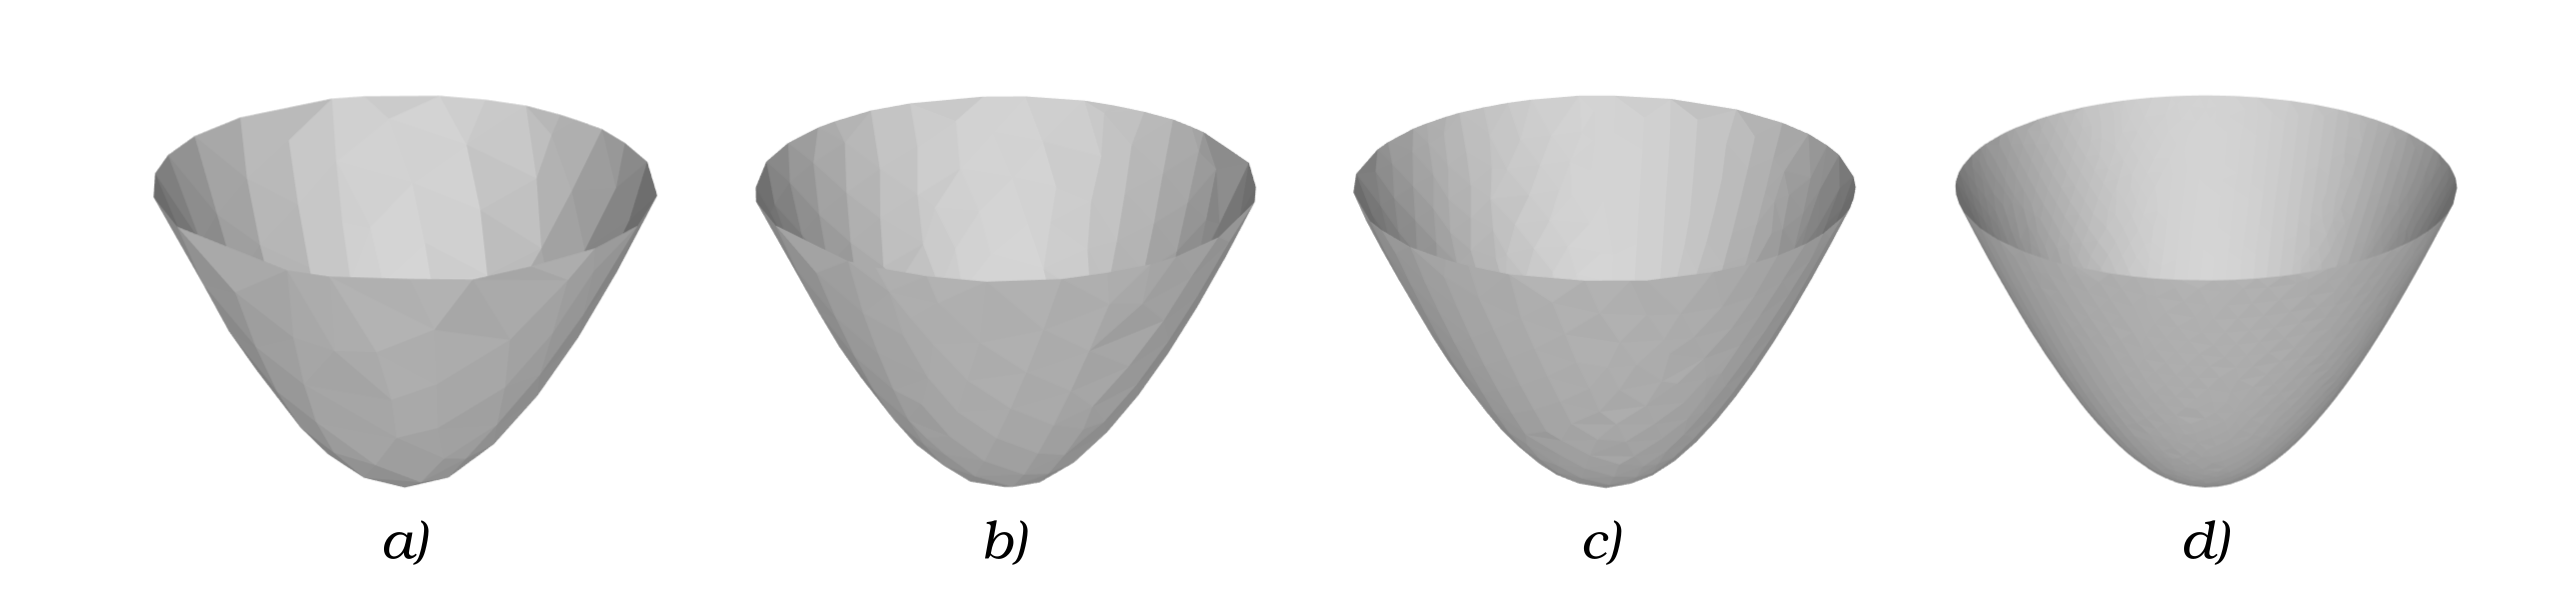
\includegraphics[width=1\textwidth]{images/elliptic_paraboloid}}
        \caption[Eliptický paraboloid]{Eliptický paraboloid}
        %id obrazku, pomocou ktoreho sa budeme na obrazok odvolavat
        \label{obr:elliptic_paraboloid}
    \end{figure}

    Výsledky merania kritérií kvality môžeme vidieť v tabuľke \ref{tab:elliptic_paraboloid}.

    \begin{table}[ht]
     \label{tab:elliptic_paraboloid}
     \caption[Výsledky merania triangulácie eliptického paraboloidu]{Výsledky merania}
        \begin{center}
            \begin{tabular}{|c|A B C D E F G H|}
                \hline
                \multicolumn{9}{|c|}{Eliptický paraboloid} \\
                \hline
                $\hspace{8mm} a \hspace{8mm}$ & $k_1$ & $k_2$ & $k_3$ & $k_4$ & $k_5$ & $k_6$ & $k_7$ & $k_8$ \EndTableHeader\\
                \hline
                1 & 0.000 & 0.029 & 0.912 & 0.9 & 0.629 & 0.049 & 0.802 & 0.802\\
                \hline
                0.75 & 0.819 & 0.027 & 0.918 & 0.9 & 0.629 & 0.049 & 0.802 & 0.802\\
                \hline
                0.5 & 0.845 & 0.024 & 0.931 & 0.9 & 0.629 & 0.049 & 0.802 & 0.802\\
                \hline
                0.25 & 0.858 & 0.021 & 0.937 & 0.9 & 0.629 & 0.049 & 0.802 & 0.802\\
                \hline
                \hline
            \end{tabular}
        \end{center}
    \end{table}

}
\newpage
\item{
    \textit{Hyperbolický paraboloid}

    \begin{equation}
    \label{eq:hyperbolic_paraboloid}
        x^2-y^2+2z = 0
    \end{equation}

    Plocha je ohraničená ohraničujúcou obálkou danou $3$-rozmerným intervalom 
    \newline
    \mbox{$\langle -3, 3 \rangle \times \langle -3, 3 \rangle \times \langle -20, 20 \rangle$}.

    Na obrázku \ref{obr:hyperbolic_paraboloid} vidíme výslednú trianguláciu hyperbolického paraboloidu
    daného implicitnou rovnicou \ref{eq:hyperbolic_paraboloid} so štyrmi rôznymi dĺžkami strany $a$.
    \begin{enumerate}[a)]
    \item{
        $a=1$, $n=$, $p=$
    }
    \item{
        $a=0.75$, $n=$, $p=$
    }
    \item{
        $a=0.5$, $n=$, $p=$
    }
    \item{
        $a=0.25$, $n=$, $p=$
    }
    \end{enumerate}

    \begin{figure}
        \centerline{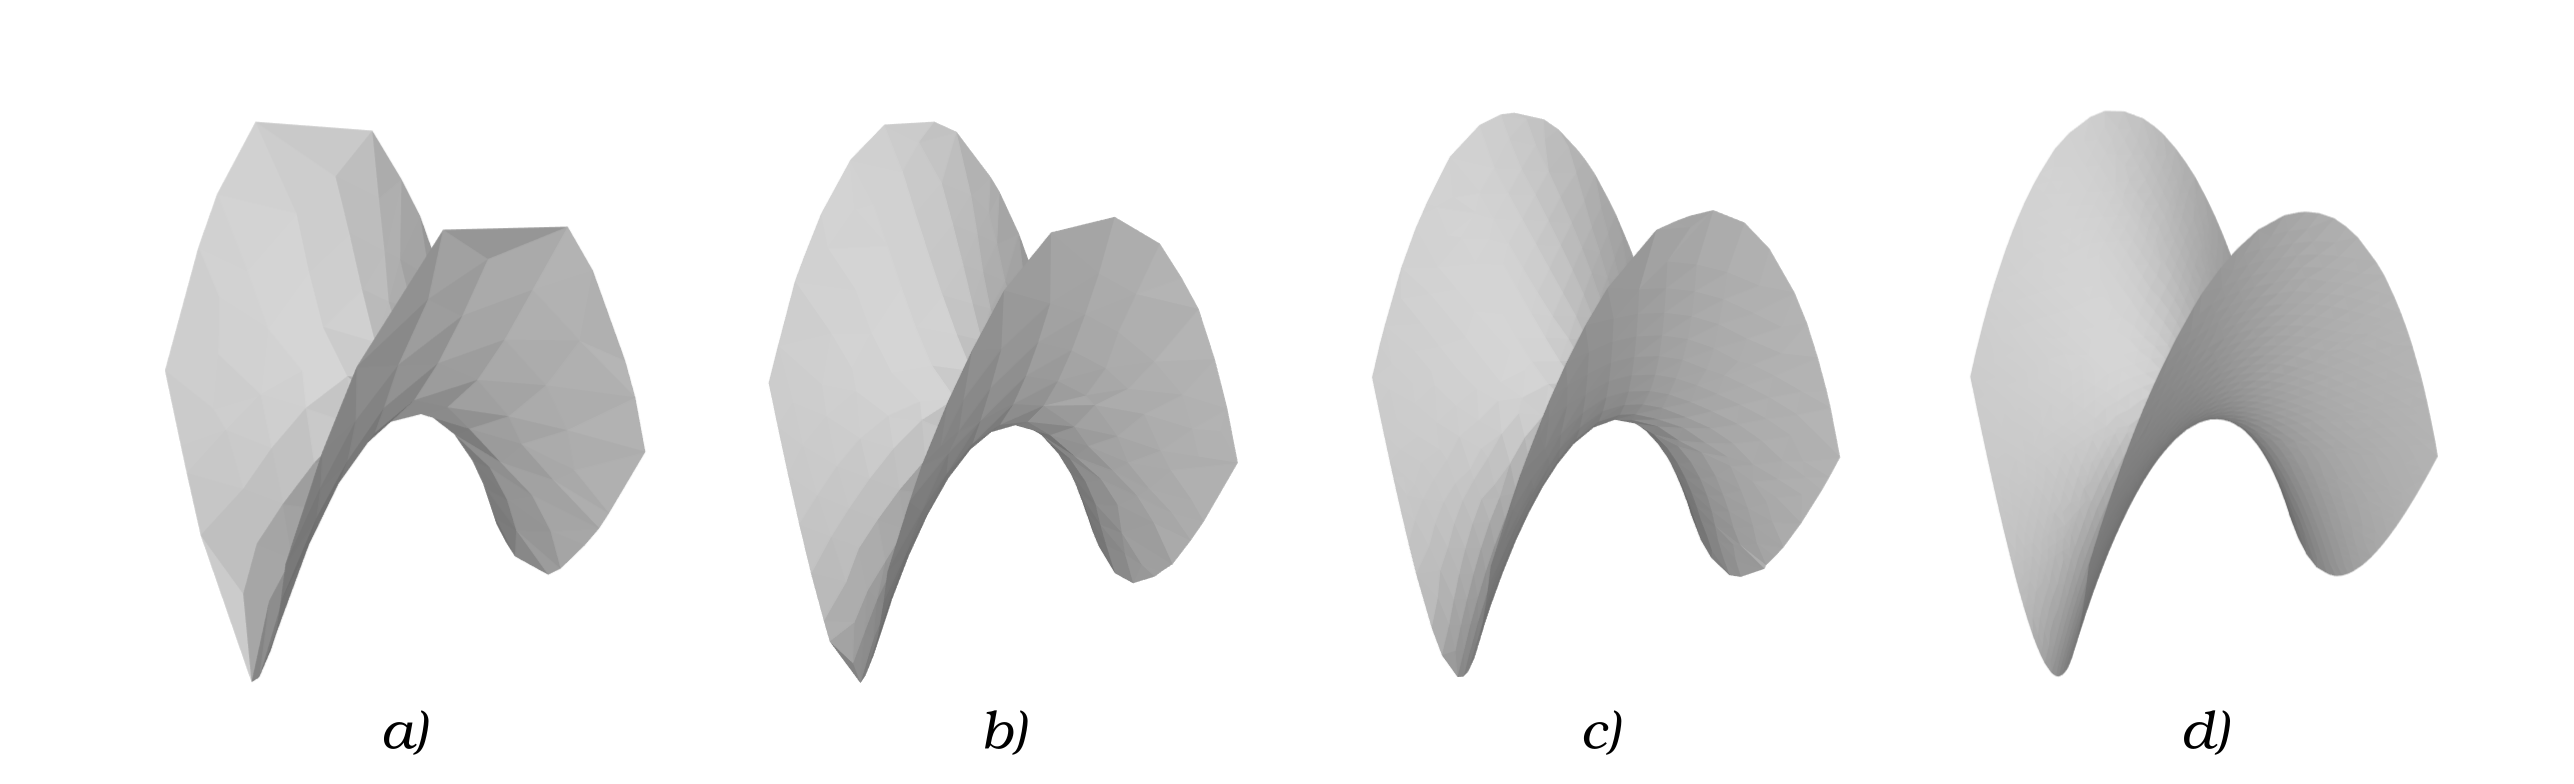
\includegraphics[width=1\textwidth]{images/hyperbolic_paraboloid}}
        \caption[Hyperbolický paraboloid]{Hyperbolický paraboloid}
        %id obrazku, pomocou ktoreho sa budeme na obrazok odvolavat
        \label{obr:hyperbolic_paraboloid}
    \end{figure}

    Výsledky merania kritérií kvality môžeme vidieť v tabuľke \ref{tab:hyperbolic_paraboloid}.

    \begin{table}[ht]
     \label{tab:hyperbolic_paraboloid}
     \caption[Výsledky merania triangulácie Hyperbolického paraboloidu]{Výsledky merania}
        \begin{center}
            \begin{tabular}{|c|A B C D E F G H|}
                \hline
                \multicolumn{9}{|c|}{Hyperbolický paraboloid} \\
                \hline
                $\hspace{8mm} a \hspace{8mm}$ & $k_1$ & $k_2$ & $k_3$ & $k_4$ & $k_5$ & $k_6$ & $k_7$ & $k_8$ \EndTableHeader\\
                \hline
                1 & 0.000 & 0.029 & 0.912 & 0.9 & 0.629 & 0.049 & 0.802 & 0.802\\
                \hline
                0.75 & 0.819 & 0.027 & 0.918 & 0.9 & 0.629 & 0.049 & 0.802 & 0.802\\
                \hline
                0.5 & 0.845 & 0.024 & 0.931 & 0.9 & 0.629 & 0.049 & 0.802 & 0.802\\
                \hline
                0.25 & 0.858 & 0.021 & 0.937 & 0.9 & 0.629 & 0.049 & 0.802 & 0.802\\
                \hline
                \hline
            \end{tabular}
        \end{center}
    \end{table}
}
\newpage
\item{
    \textit{Parabolický cylinder (??)}

    \begin{equation}
    \label{eq:parabolic_cylinder}
        x^2+2y = 0
    \end{equation}

    Plocha je ohraničená ohraničujúcou obálkou danou $3$-rozmerným intervalom 
    \newline
    \mbox{$\langle -5, 5 \rangle \times \langle -5, 5 \rangle \times \langle -5, 5 \rangle$}.

    Na obrázku \ref{obr:parabolic_cylinder} vidíme výslednú trianguláciu parabolického cylindra
    daného implicitnou rovnicou \ref{eq:parabolic_cylinder} so štyrmi rôznymi dĺžkami strany $a$.
    \begin{enumerate}[a)]
    \item{
        $a=1$, $n=$, $p=$
    }
    \item{
        $a=0.75$, $n=$, $p=$
    }
    \item{
        $a=0.5$, $n=$, $p=$
    }
    \item{
        $a=0.25$, $n=$, $p=$
    }
    \end{enumerate}

    \begin{figure}
        \centerline{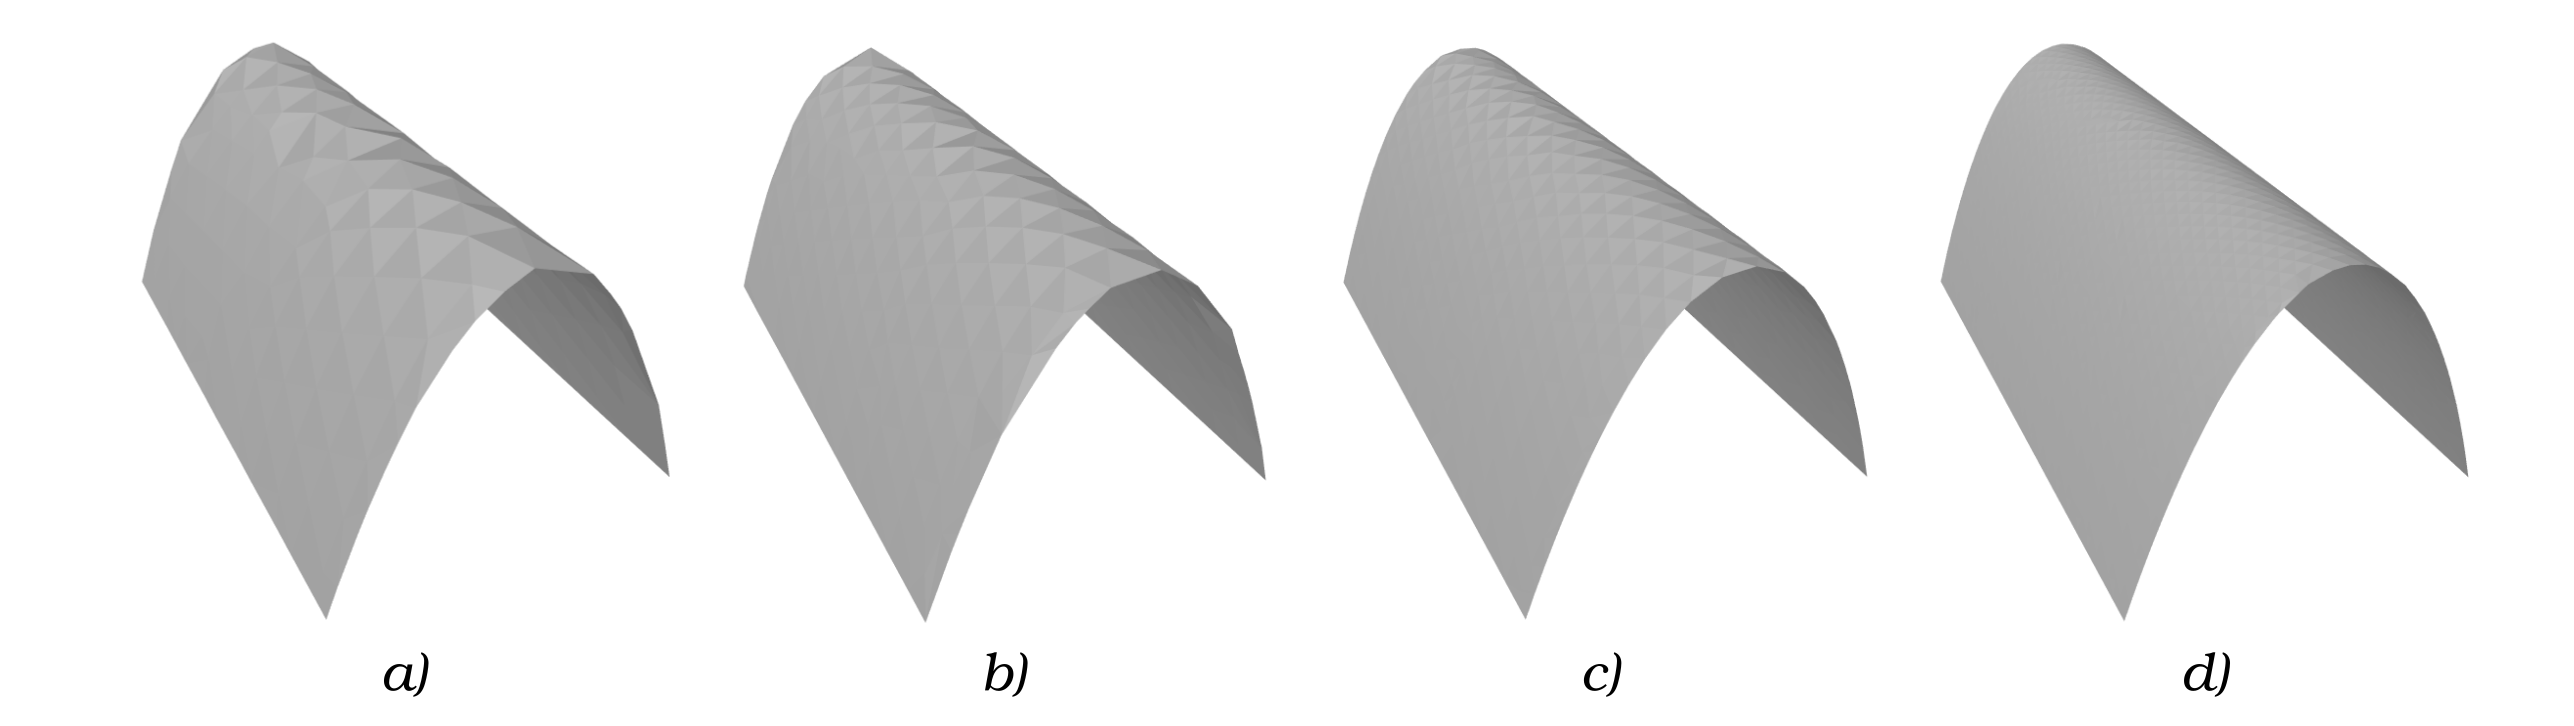
\includegraphics[width=1\textwidth]{images/parabolic_cylinder}}
        \caption[Parabolický cylinder]{Parabolický cylinder}
        %id obrazku, pomocou ktoreho sa budeme na obrazok odvolavat
        \label{obr:parabolic_cylinder}
    \end{figure}

    Výsledky merania kritérií kvality môžeme vidieť v tabuľke \ref{tab:parabolic_cylinder}.

    \begin{table}[ht]
     \label{tab:parabolic_cylinder}
     \caption[Výsledky merania triangulácie parabolického cylindra]{Výsledky merania}
        \begin{center}
            \begin{tabular}{|c|A B C D E F G H|}
                \hline
                \multicolumn{9}{|c|}{Parabolický cylinder} \\
                \hline
                $\hspace{8mm} a \hspace{8mm}$ & $k_1$ & $k_2$ & $k_3$ & $k_4$ & $k_5$ & $k_6$ & $k_7$ & $k_8$ \EndTableHeader\\
                \hline
                1 & 0.000 & 0.029 & 0.912 & 0.9 & 0.629 & 0.049 & 0.802 & 0.802\\
                \hline
                0.75 & 0.819 & 0.027 & 0.918 & 0.9 & 0.629 & 0.049 & 0.802 & 0.802\\
                \hline
                0.5 & 0.845 & 0.024 & 0.931 & 0.9 & 0.629 & 0.049 & 0.802 & 0.802\\
                \hline
                0.25 & 0.858 & 0.021 & 0.937 & 0.9 & 0.629 & 0.049 & 0.802 & 0.802\\
                \hline
                \hline
            \end{tabular}
        \end{center}
    \end{table}
}
\newpage
\item{
    \textit{Kvadrický kužeľ (??)}

    \begin{equation}
    \label{eq:quadric_cone}
        x^2-y^2+2*z = 0
    \end{equation}

    Plocha je ohraničená ohraničujúcou obálkou danou $3$-rozmerným intervalom 
    \newline
    \mbox{$\langle -10, 10 \rangle \times \langle -10, 10 \rangle \times \langle 1, 5 \rangle$}.

    Na obrázku \ref{obr:quadric_cone} vidíme výslednú trianguláciu kvadrického kužeľa
    daného implicitnou rovnicou \ref{eq:quadric_cone} so štyrmi rôznymi dĺžkami strany $a$.
    \begin{enumerate}[a)]
    \item{
        $a=1$, $n=$, $p=$
    }
    \item{
        $a=0.75$, $n=$, $p=$
    }
    \item{
        $a=0.5$, $n=$, $p=$
    }
    \item{
        $a=0.25$, $n=$, $p=$
    }
    \end{enumerate}

    \begin{figure}
        \centerline{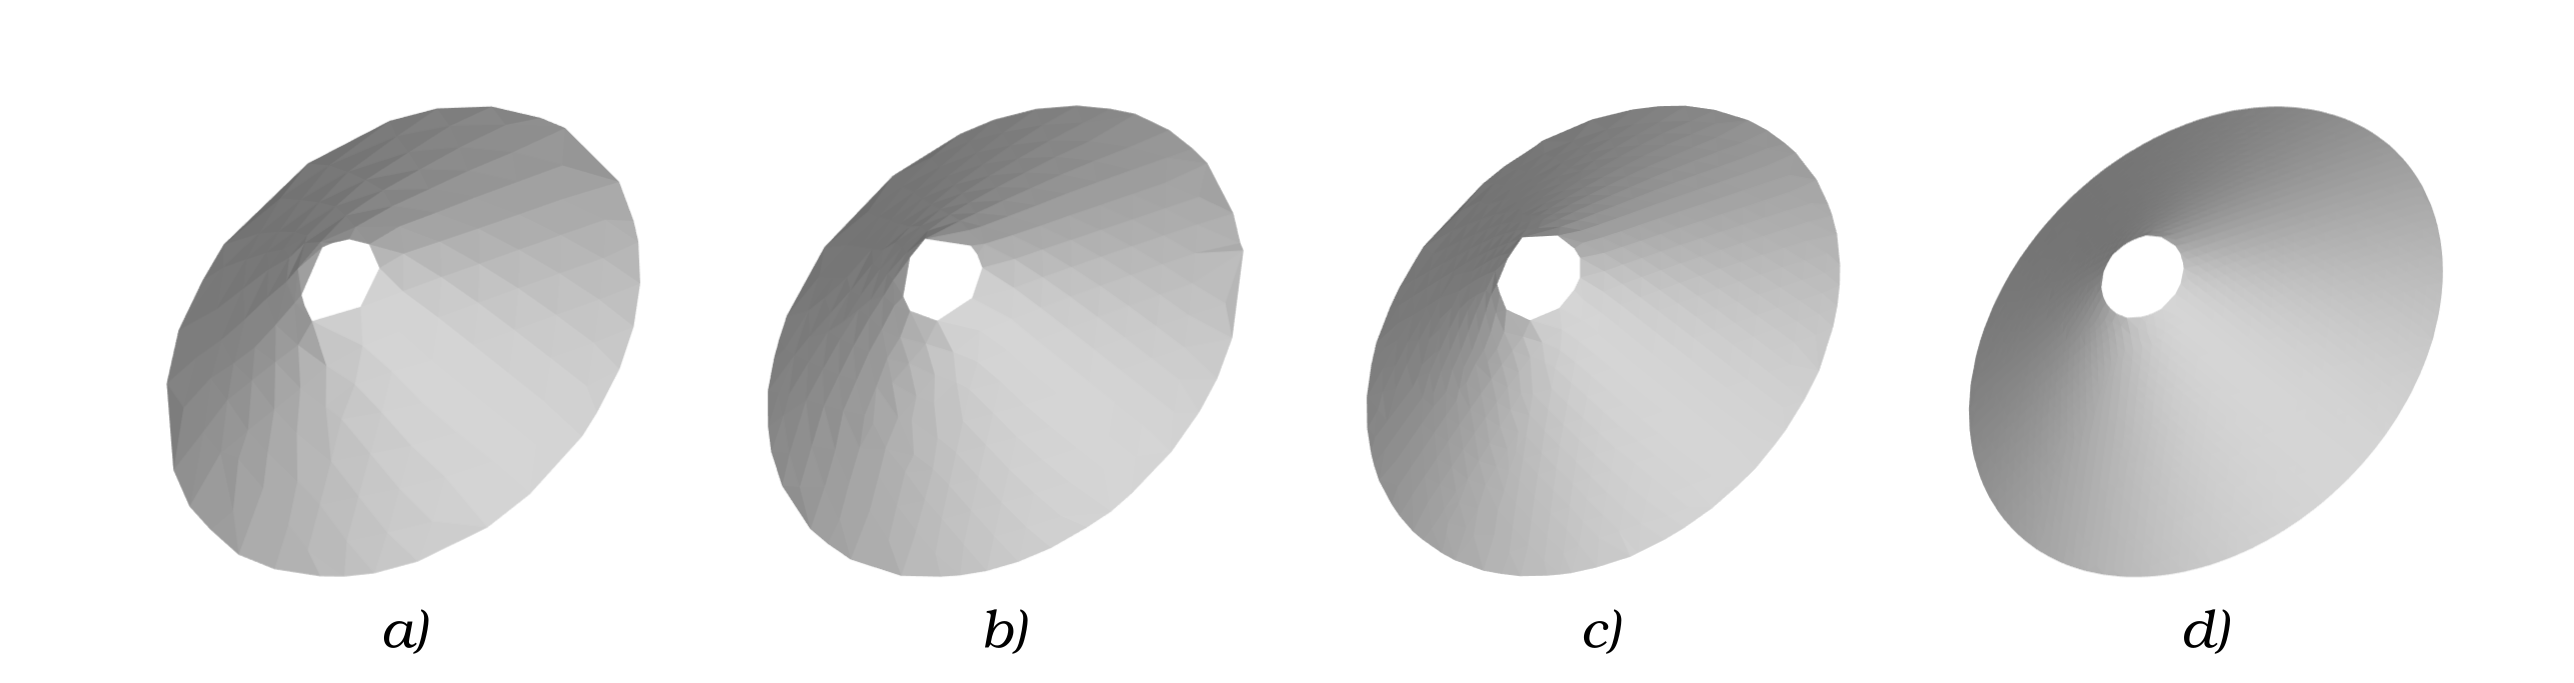
\includegraphics[width=1\textwidth]{images/quadric_cone}}
        \caption[Kvadrický kužeľ]{Kvadrický kužeľ}
        %id obrazku, pomocou ktoreho sa budeme na obrazok odvolavat
        \label{obr:quadric_cone}
    \end{figure}

    Výsledky merania kritériu kvality môžeme vidieť v tabuľke \ref{tab:quadric_cone}.

    \begin{table}[ht]
     \label{tab:quadric_cone}
     \caption[Výsledky merania triangulácie kvadrického kužeľa]{Výsledky merania}
        \begin{center}
            \begin{tabular}{|c|A B C D E F G H|}
                \hline
                \multicolumn{9}{|c|}{Kvadrický kužeľ} \\
                \hline
                $\hspace{8mm} a \hspace{8mm}$ & $k_1$ & $k_2$ & $k_3$ & $k_4$ & $k_5$ & $k_6$ & $k_7$ & $k_8$ \EndTableHeader\\
                \hline
                1 & 0.000 & 0.029 & 0.912 & 0.9 & 0.629 & 0.049 & 0.802 & 0.802\\
                \hline
                0.75 & 0.819 & 0.027 & 0.918 & 0.9 & 0.629 & 0.049 & 0.802 & 0.802\\
                \hline
                0.5 & 0.845 & 0.024 & 0.931 & 0.9 & 0.629 & 0.049 & 0.802 & 0.802\\
                \hline
                0.25 & 0.858 & 0.021 & 0.937 & 0.9 & 0.629 & 0.049 & 0.802 & 0.802\\
                \hline
                \hline
            \end{tabular}
        \end{center}
    \end{table}
}
\newpage
\item{
    \textit{Hyperboloid jedného plátu}

    \begin{equation}
    \label{eq:hyperboloid}
        x^2-y^2+2*z = 0
    \end{equation}

    Plocha je ohraničená ohraničujúcou obálkou danou $3$-rozmerným intervalom 
    \newline
    \mbox{$\langle -5, 5 \rangle \times \langle -5, 5 \rangle \times \langle -2, 2 \rangle$}.

    Na obrázku \ref{obr:hyperboloid} vidíme výslednú trianguláciu hyperboloidu
    daného implicitnou rovnicou \ref{eq:hyperboloid} so štyrmi rôznymi dĺžkami strany $a$.
    \begin{enumerate}[a)]
    \item{
        $a=1$, $n=$, $p=$
    }
    \item{
        $a=0.75$, $n=$, $p=$
    }
    \item{
        $a=0.5$, $n=$, $p=$
    }
    \item{
        $a=0.25$, $n=$, $p=$
    }
    \end{enumerate}

    \begin{figure}
        \centerline{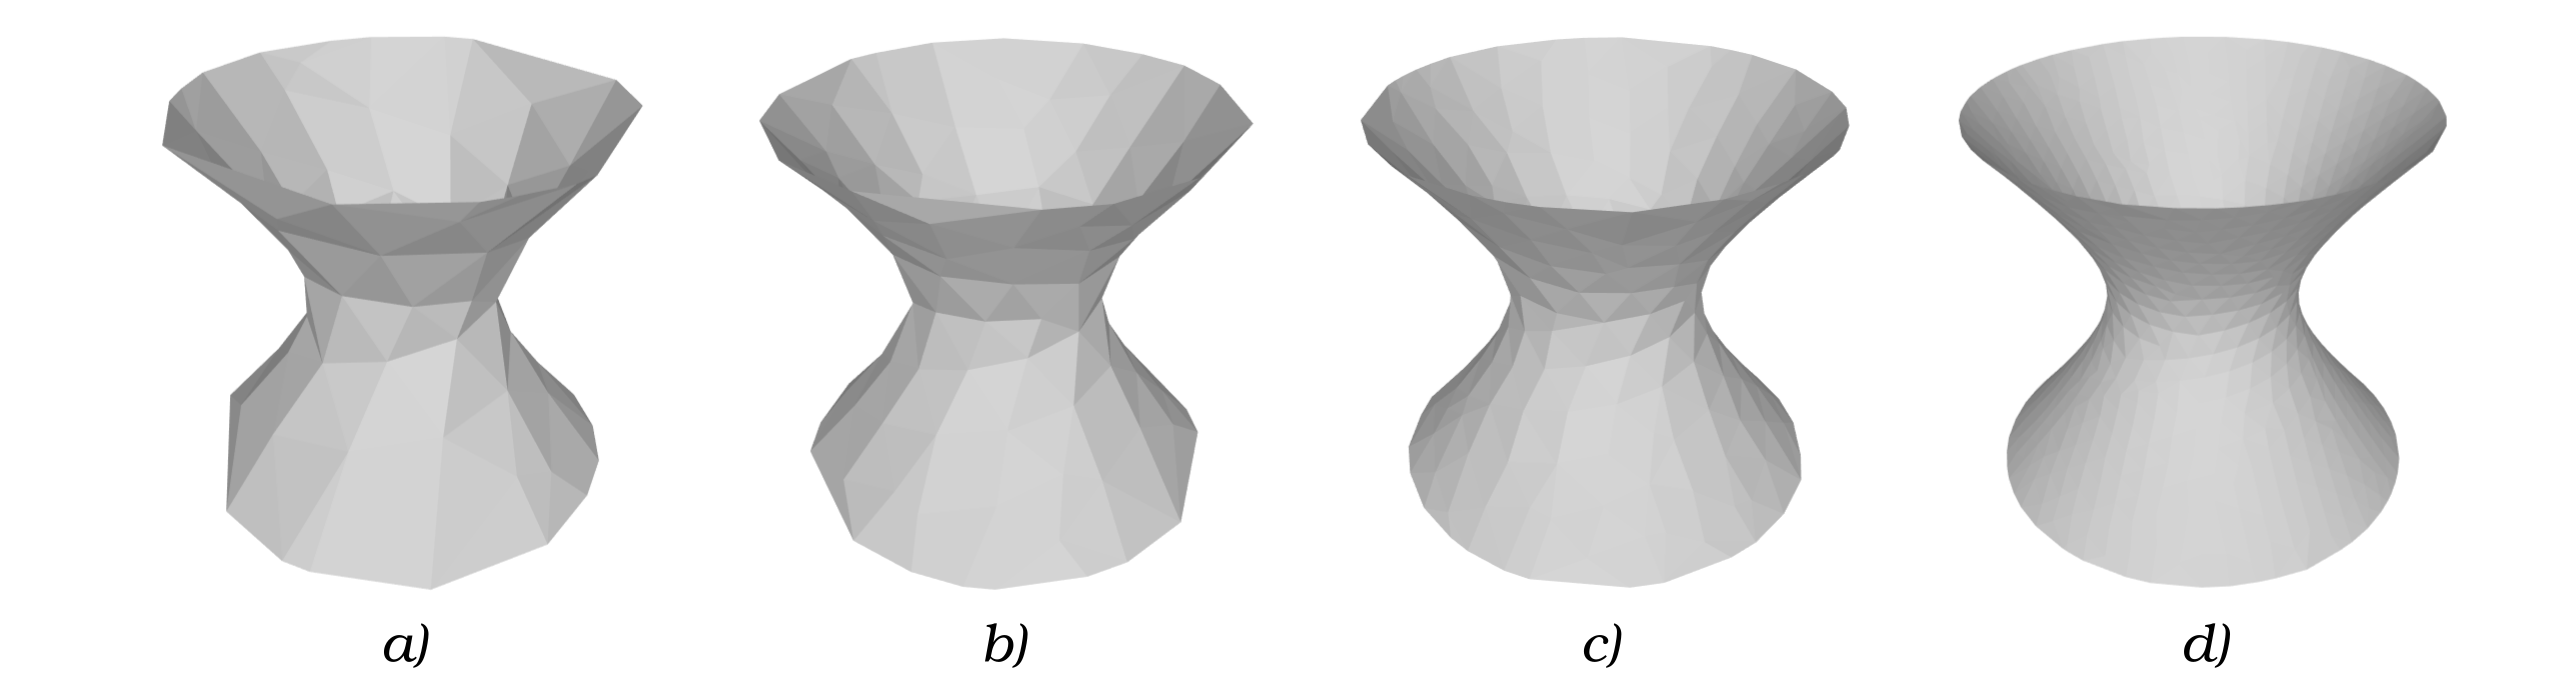
\includegraphics[width=1\textwidth]{images/hyperboloid}}
        \caption[Hyperboloid]{Hyperboloid}
        %id obrazku, pomocou ktoreho sa budeme na obrazok odvolavat
        \label{obr:hyperboloid}
    \end{figure}

    Výsledky merania kritérií kvality môžeme vidieť v tabuľke \ref{tab:hyperboloid}.

    \begin{table}[ht]
     \label{tab:hyperboloid}
     \caption[Výsledky merania triangulácie hyperboloidu]{Výsledky merania}
        \begin{center}
            \begin{tabular}{|c|A B C D E F G H|}
                \hline
                \multicolumn{9}{|c|}{Hyperboloid} \\
                \hline
                $\hspace{8mm} a \hspace{8mm}$ & $k_1$ & $k_2$ & $k_3$ & $k_4$ & $k_5$ & $k_6$ & $k_7$ & $k_8$ \EndTableHeader\\
                \hline
                1 & 0.000 & 0.029 & 0.912 & 0.9 & 0.629 & 0.049 & 0.802 & 0.802\\
                \hline
                0.75 & 0.819 & 0.027 & 0.918 & 0.9 & 0.629 & 0.049 & 0.802 & 0.802\\
                \hline
                0.5 & 0.845 & 0.024 & 0.931 & 0.9 & 0.629 & 0.049 & 0.802 & 0.802\\
                \hline
                0.25 & 0.858 & 0.021 & 0.937 & 0.9 & 0.629 & 0.049 & 0.802 & 0.802\\
                \hline
                \hline
            \end{tabular}
        \end{center}
    \end{table}
}
\end{enumerate}

\newpage

\subsection{Ohraničenie}

V kapitole \ref{kap:important_methods} sme opísali dva spôsoby orezávania na ohraničujúcu obálku.
Prvý spôsob orezávanie je pripínanie na najbližší bod ohraničujúcej obálky, teda v smere normály 
niektorej zo stien tejto obálky. Druhý spôsob je v smere ťažnice trojuholníka. Oba spôsoby demonštrujeme obrázkami
a slovne popíšeme naše pozorovania.

Na obrázku \ref{obr:cut_sphere_normal} môžeme vidieť trianguláciu zrezanej sféry pre 4 rôzne dĺžky 
hrany $a$, kde je orezávanie docielené pripínaním na najbližší bod obálky. Vidíme, že na stenách obálky 
je triangulácia veľmi nepresná.

\begin{figure}
    \centerline{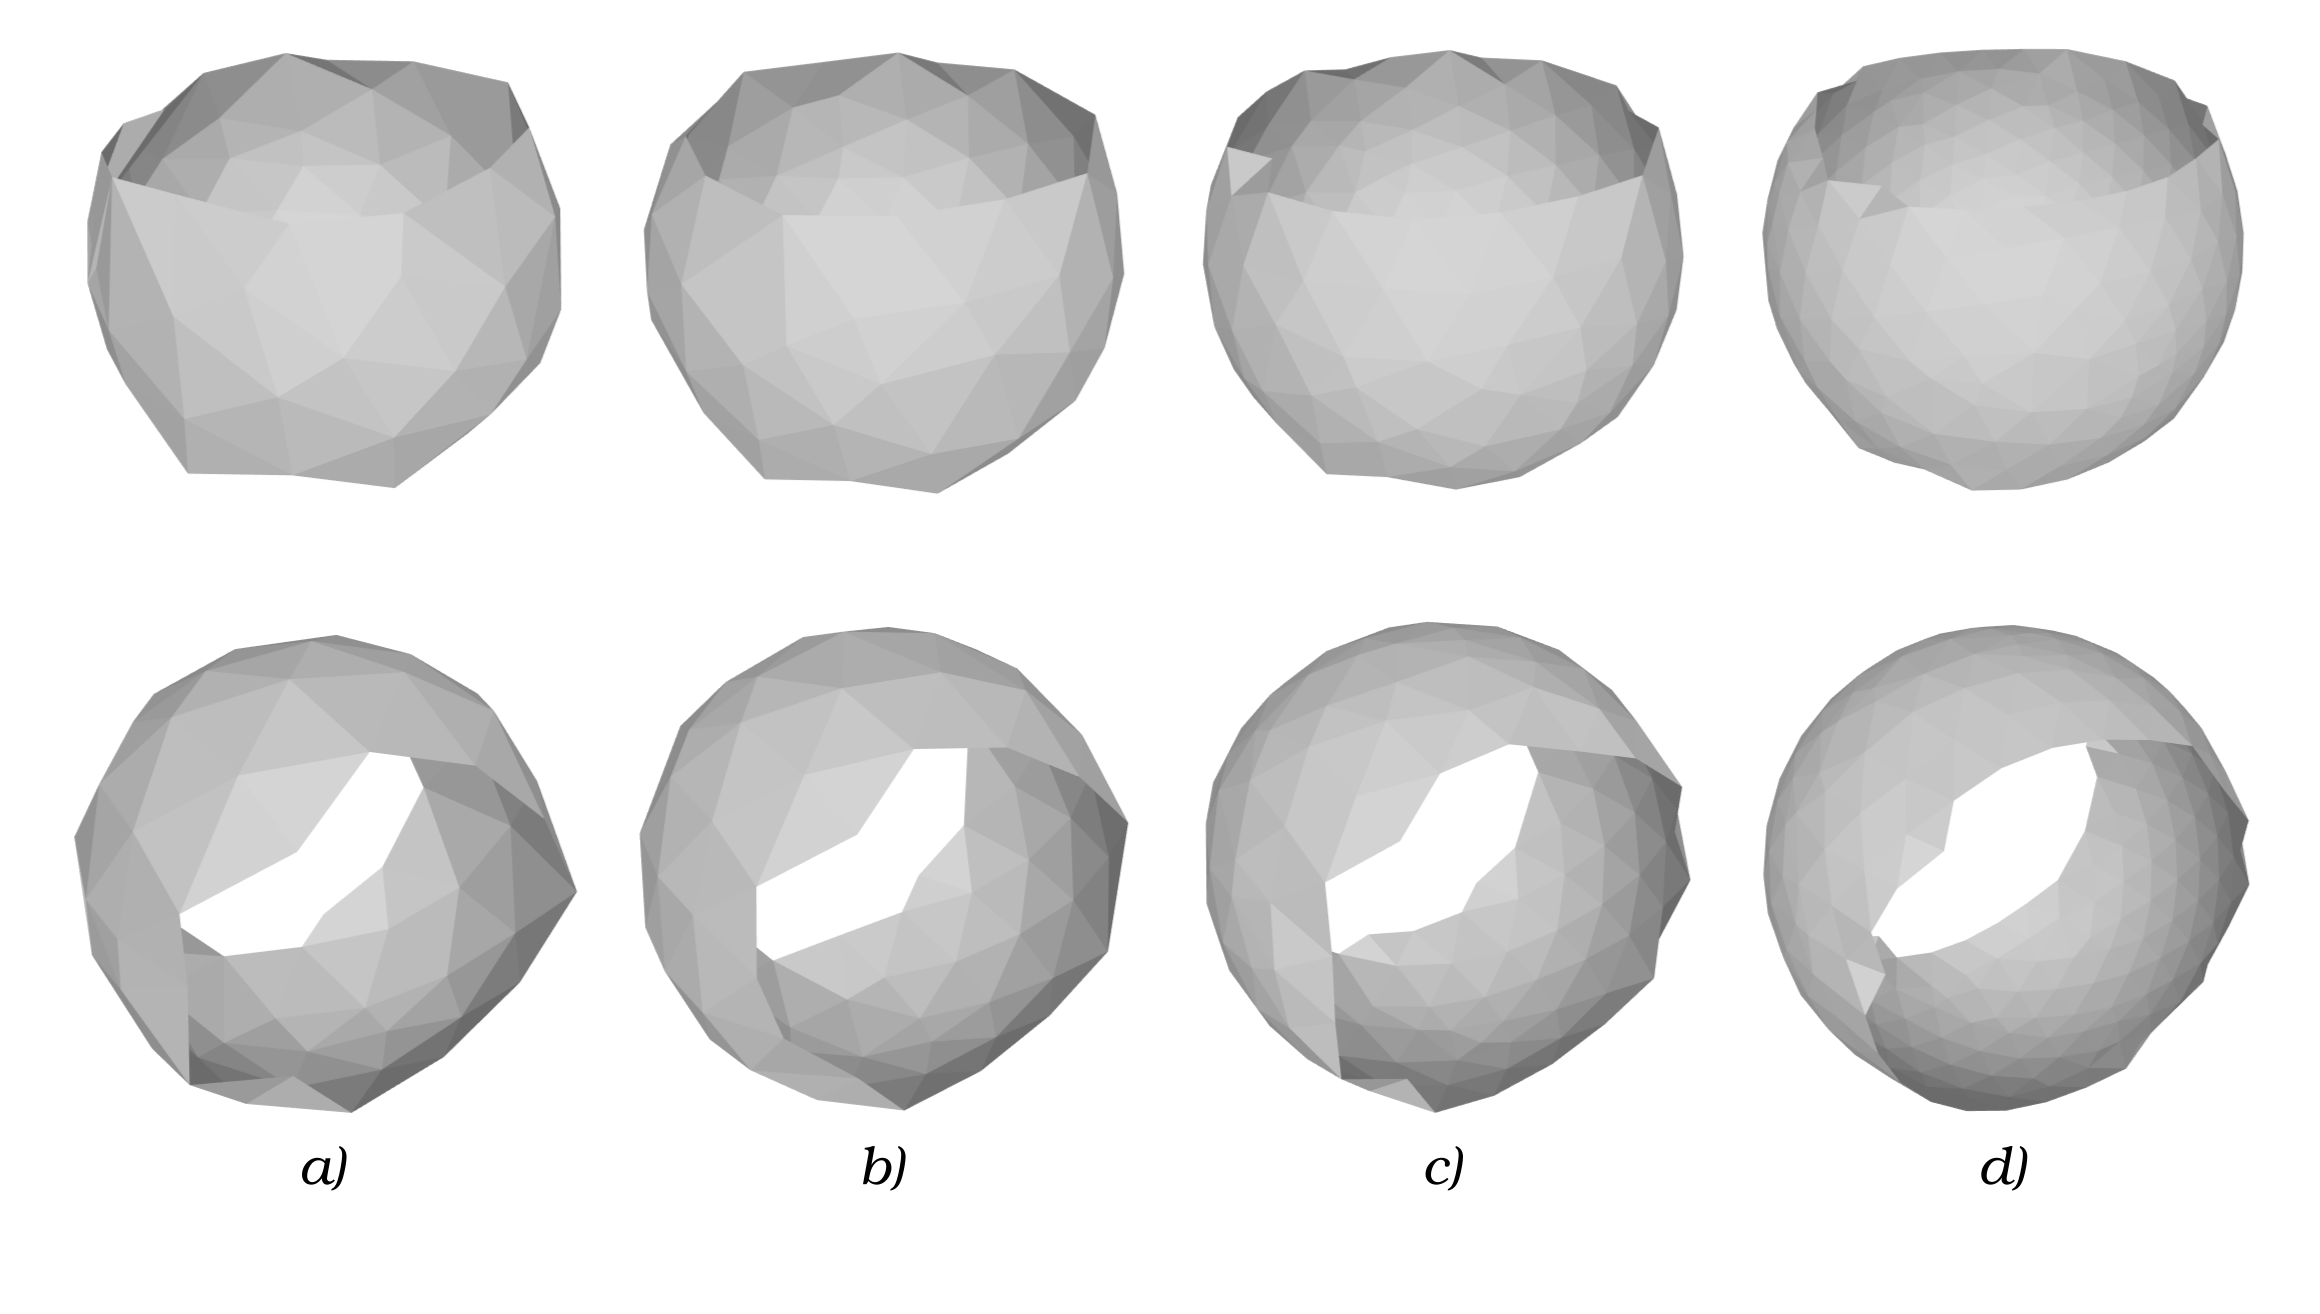
\includegraphics[width=0.8\textwidth]{images/cut_sphere_normal}}
    \caption[Ohraničená triangulácia gule -- premietanie na najbližší bod]
    {Premietanie na najbližší bod.}
    %id obrazku, pomocou ktoreho sa budeme na obrazok odvolavat
    \label{obr:cut_sphere_normal}
\end{figure}

Na obrázku \ref{obr:cut_sphere} môžeme naopak vidieť trianguláciu rovnakej zrezanej sféry s rovnakými 
dĺžkami hrany $a$.
Vidíme, že triangulácia vyzerá omnoho presnejšie a prirodzenejšie.

\begin{figure}
    \centerline{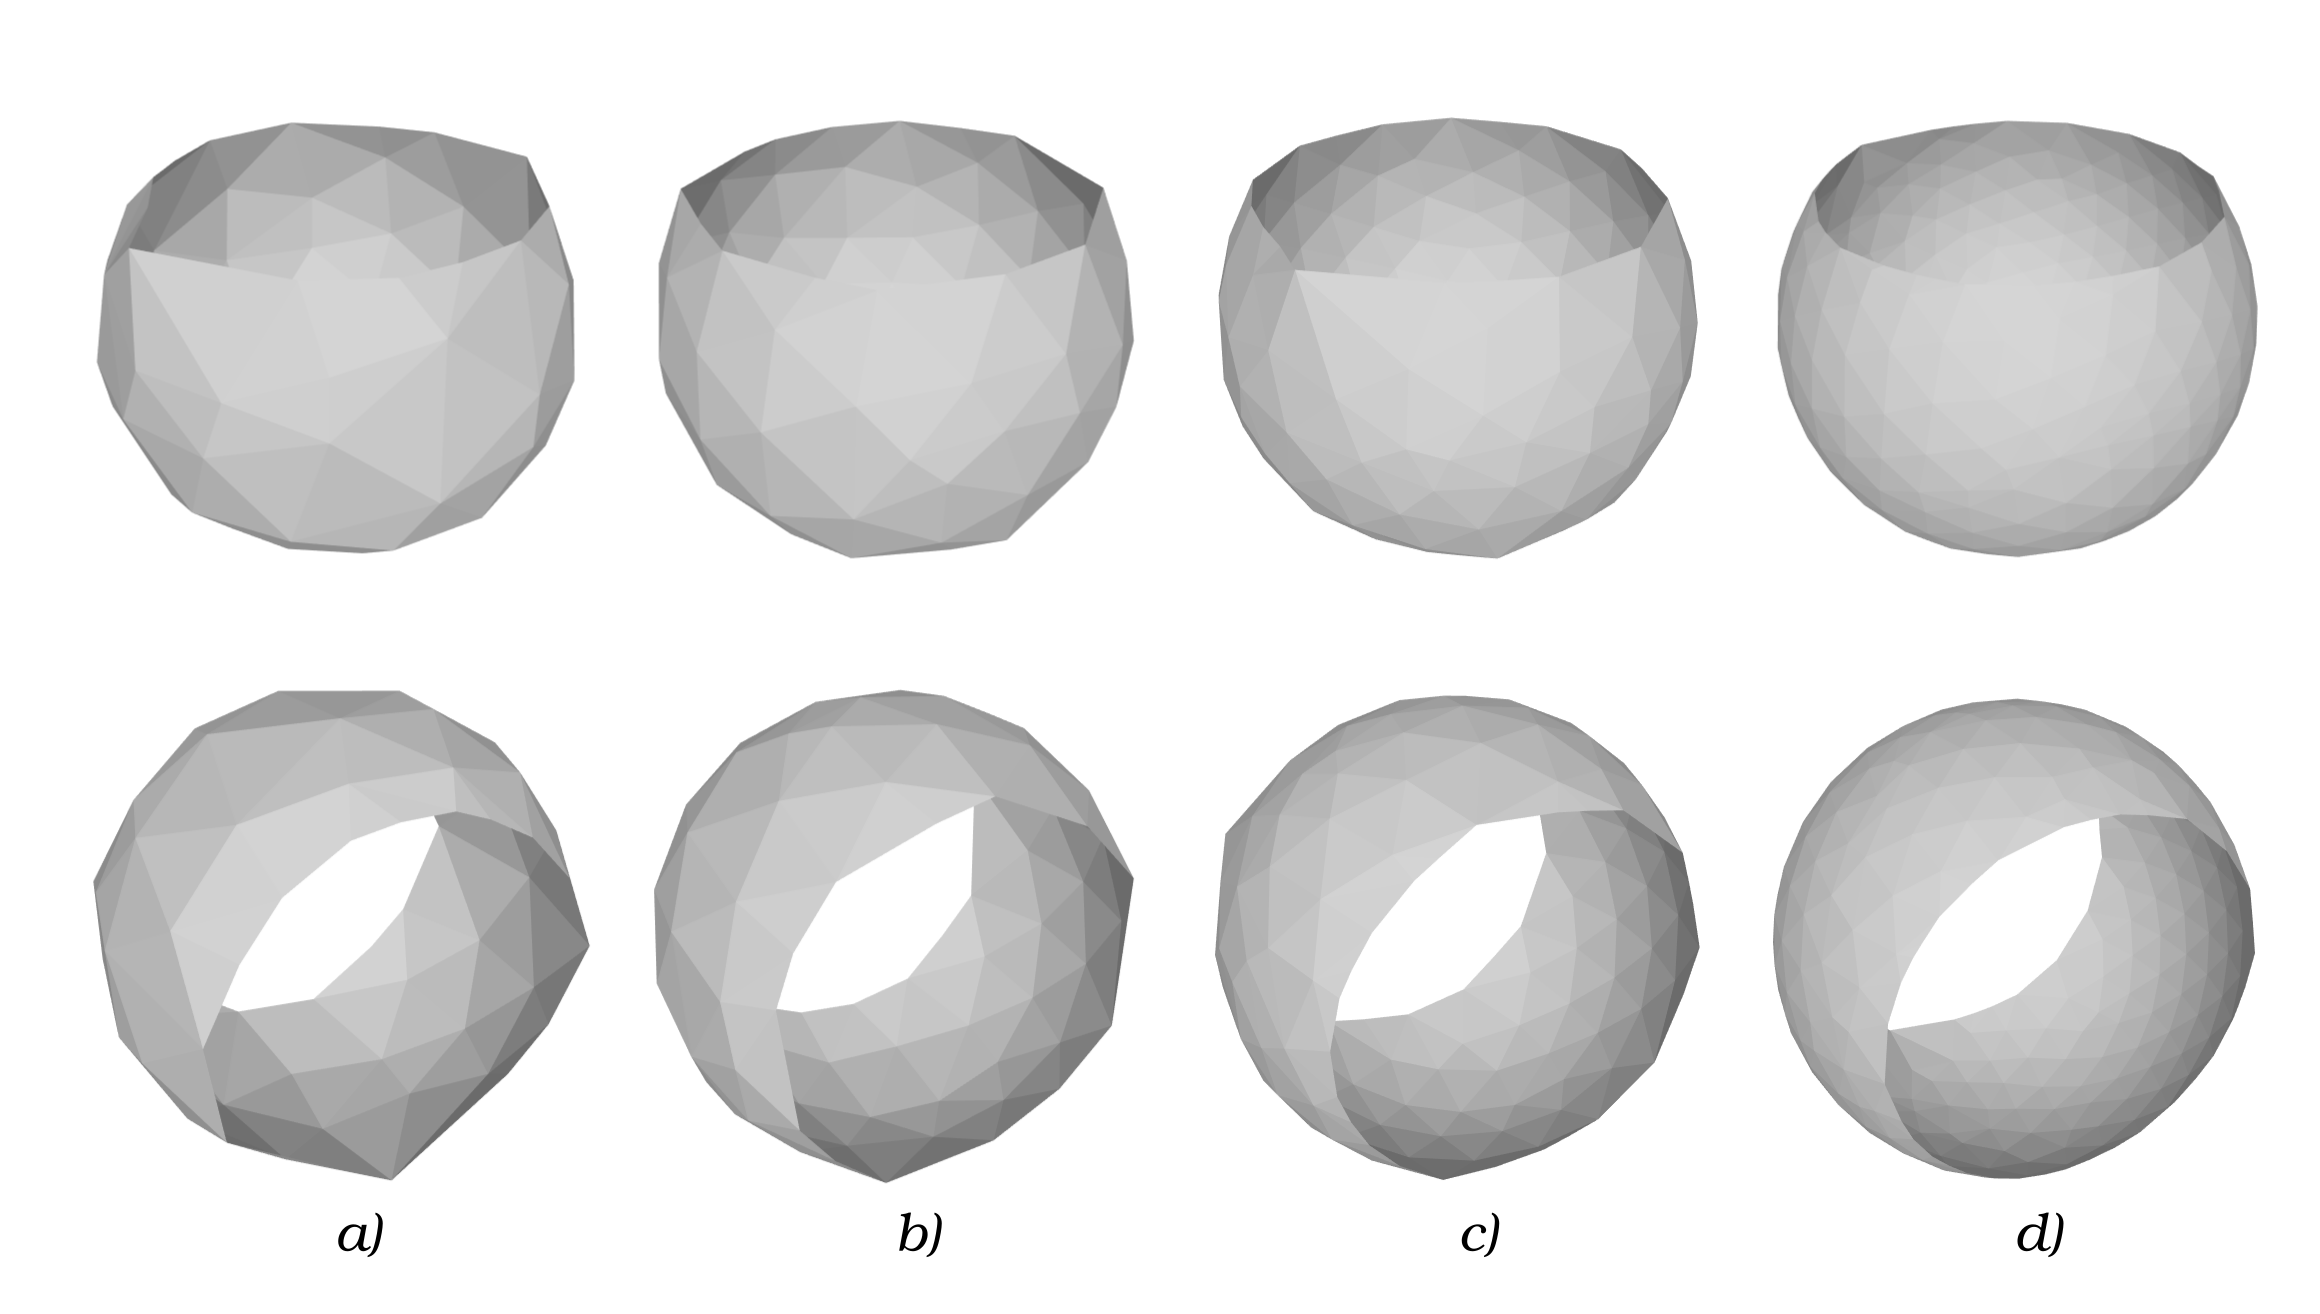
\includegraphics[width=0.8\textwidth]{images/cut_sphere}}
    \caption[Ohraničená triangulácia gule -- premietanie v smere ťažnice]
    {Premietanie v smere ťažnice.}
    %id obrazku, pomocou ktoreho sa budeme na obrazok odvolavat
    \label{obr:cut_sphere}
\end{figure}

Nie je však pravda, že pripínanie na obálky v smere ťažnice je vždy lepšie.
Pripínanie v smere ťažnice má nevýhodu vytváranie užších trojuholníkov pri 
okraji. Pripínanie na najbližší bod má zase nevýhodu, že smer premietania
nie je vždy v smere podobnom dotyčnice plochy.
Niektoré plochy však nemajú takúto nevýhodu.
Sú to plochy, ktoré majú v mieste orezania dotyčnicu približne v smere normály.
Pre takéto plochy býva prichytávanie v smere normály kvalitnejšie ako 
prichytávanie v smere ťažnice.

Toto správanie môžeme vidieť na obrázku \ref{obr:cylinder} a obrázku \ref{obr:cylinder_normal}, 
os valca je rovnobežná s jednou zo súradnicových osí.

Na obrázku \ref{obr:cylinder} vidíme orezaný valec, pričom používame
pripínanie v smere ťažnice. Na okraji môžeme vidieť užšie trojuholníky. 
Kdežto na obrázku \ref{obr:cylinder_normal} vidíme ten istý valec, 
avšak na pripínanie používame pripínanie k najbližšiemu bodu obálky.
Vidíme že tento valec nemá na okraji veľmi úzke trojuholníky avšak 
nemá ani deformovaný okraj ako sme to videli pri orezanej sfére.

\begin{figure}
    \centerline{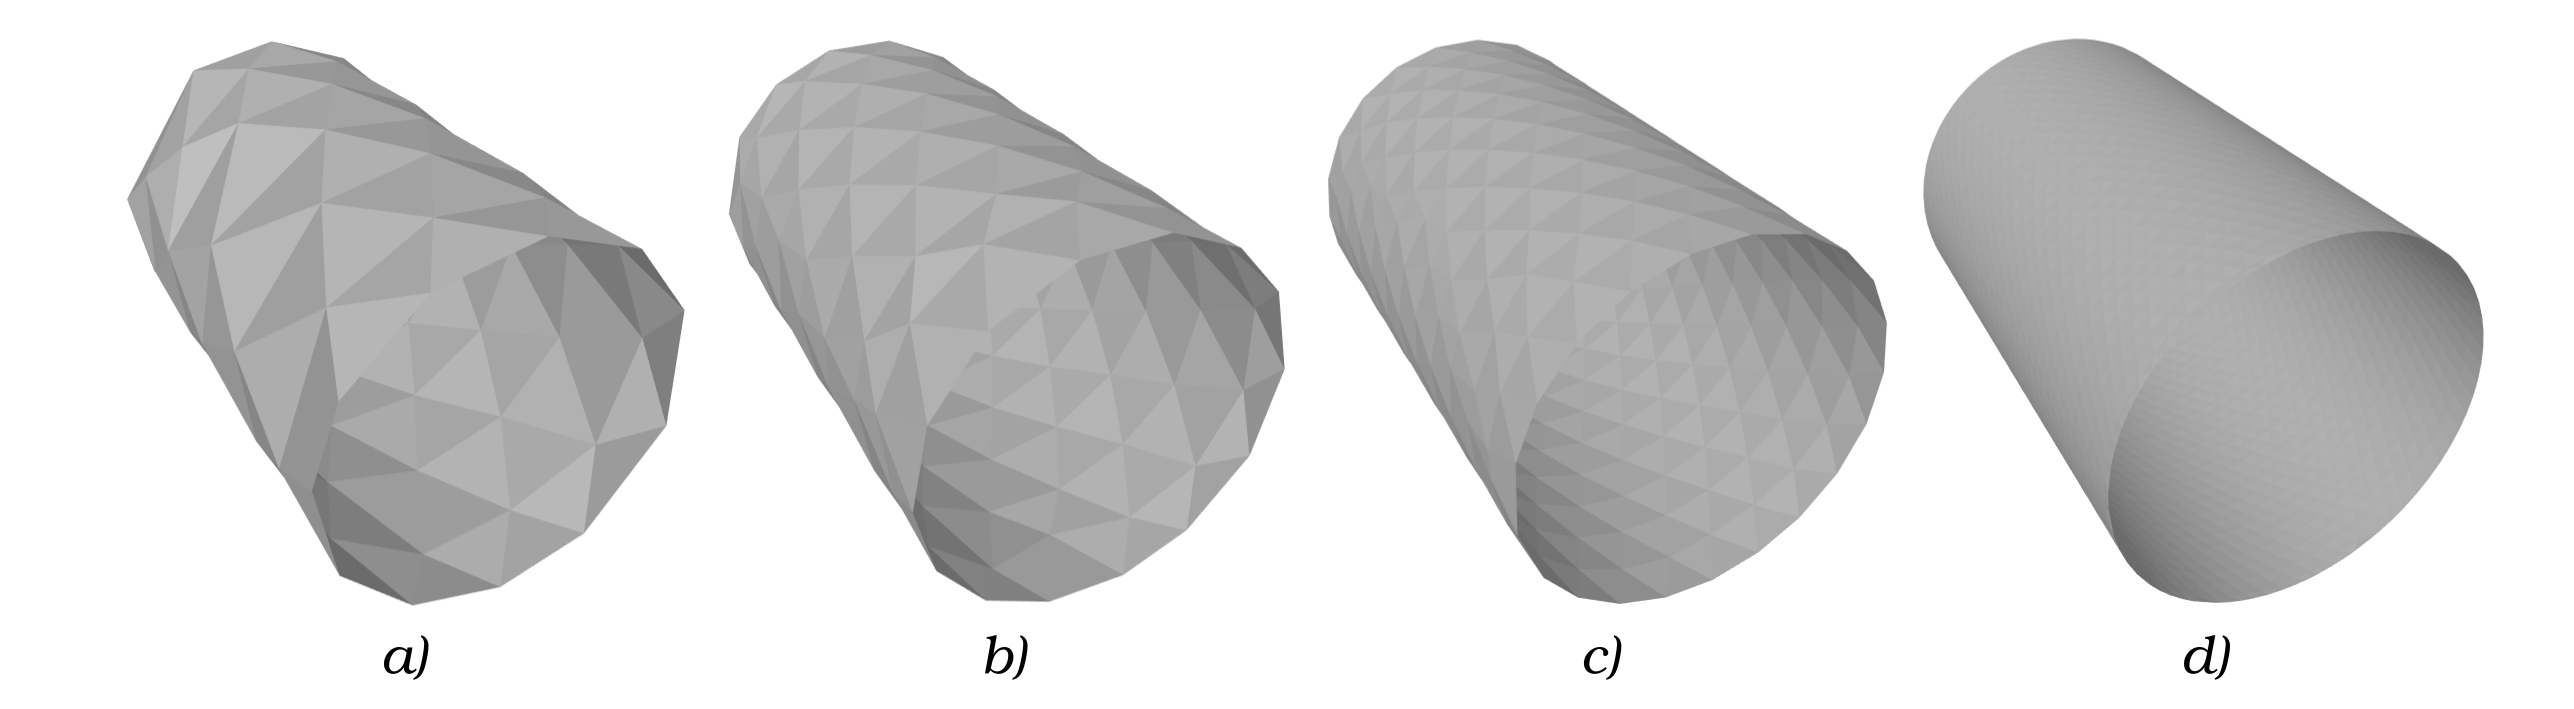
\includegraphics[width=1\textwidth]{images/cylinder_normal}}
    \caption[Ohraničená triangulácia tetrahedronu -- premietanie na najbližší bod]
    {Premietanie v smere ťažnice.}
    %id obrazku, pomocou ktoreho sa budeme na obrazok odvolavat
    \label{obr:cylinder_normal}
\end{figure}

\begin{figure}
    \centerline{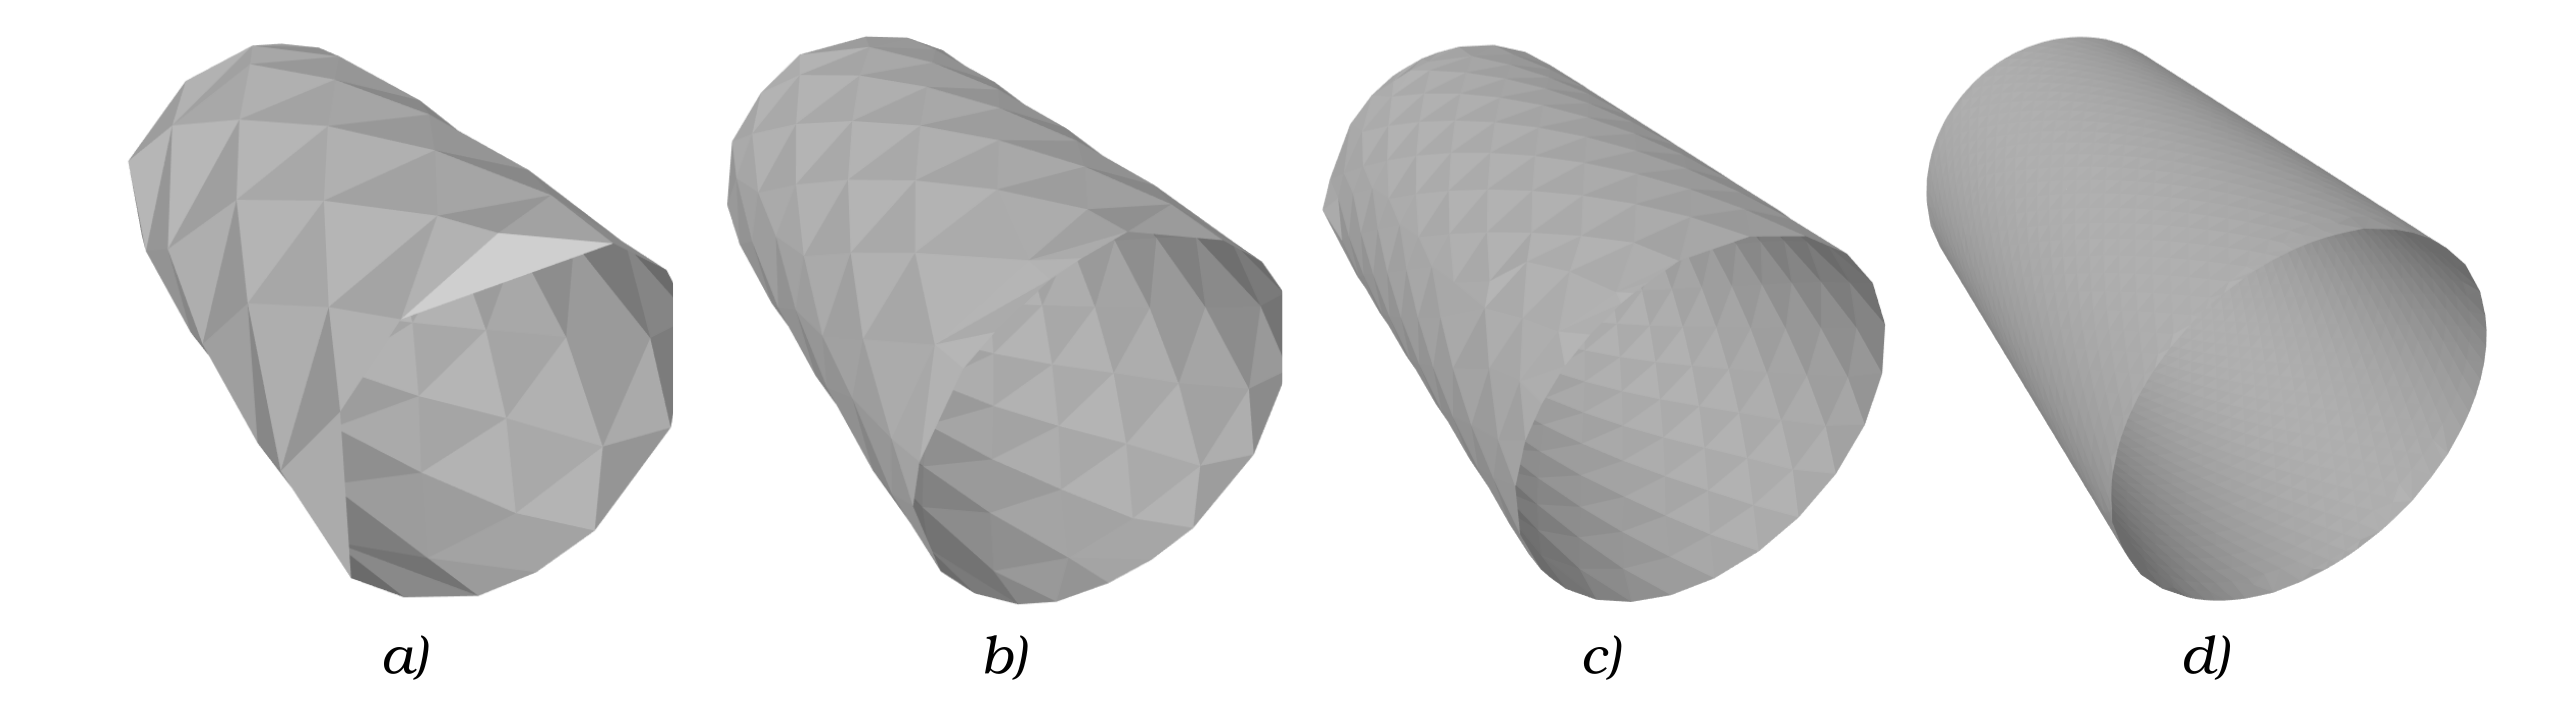
\includegraphics[width=1\textwidth]{images/cylinder}}
    \caption[Ohraničená triangulácia tetrahedronu -- premietanie v smere ťažnice]
    {Premietanie v smere ťažnice.}
    %id obrazku, pomocou ktoreho sa budeme na obrazok odvolavat
    \label{obr:cylinder}
\end{figure}

\section{Adaptívna triangulácia}
\subsection{Prerozdeľovanie trojuholníkov}

V našej práci sme implementovali jednu iteráciu adaptívneho prerozdelenia trojuholníkov
na miestach kde je ťažisko trojuholníka od plochy vzdialenejšie ako zvolená prahová hodnota $d$.

Na obrázku \ref{obr:adaptive_ellipsoid} vidíme trianguláciu elipsoidu so zvolenou dĺžkou hrany $a=0.7$.

\begin{figure}
    \centerline{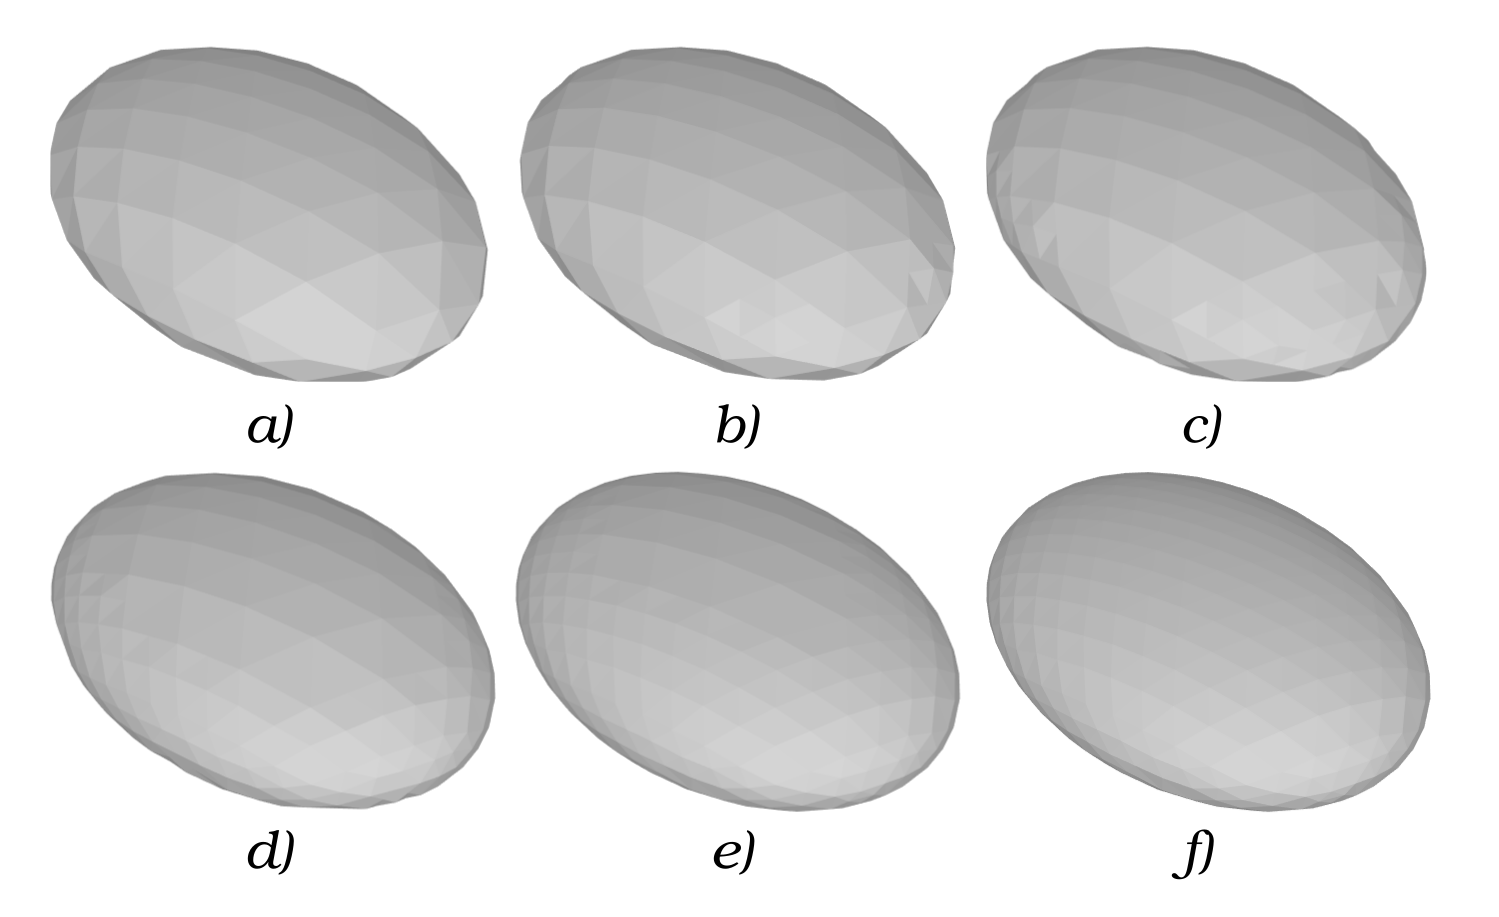
\includegraphics[width=0.6\textwidth]{images/adaptive_ellipsoid}}
    \caption[Adaptívne prerozdelenie elipsoidu.]
    {$a)$ bez adaptívneho prerozdelenia, $b)$ $d=0.05$, $c)$ $d=0.04$, $d)$ $d=0.03$, $e)$ $d=0.02$, $f)$ $d=0.01$}
    %id obrazku, pomocou ktoreho sa budeme na obrazok odvolavat
    \label{obr:adaptive_ellipsoid}
\end{figure}


Toto adaptívne prerozdelenie sme vyskúšali aj na nekonečnej ploche.
Na obrázku \ref{obr:adaptive_parabolic_cylinder} vidíme trianguláciu parabolického 
cylindra so zvolenou dĺžkou hrany $a=2$ a rôznymi prahovými hodnotami $d$.

\begin{figure}
    \centerline{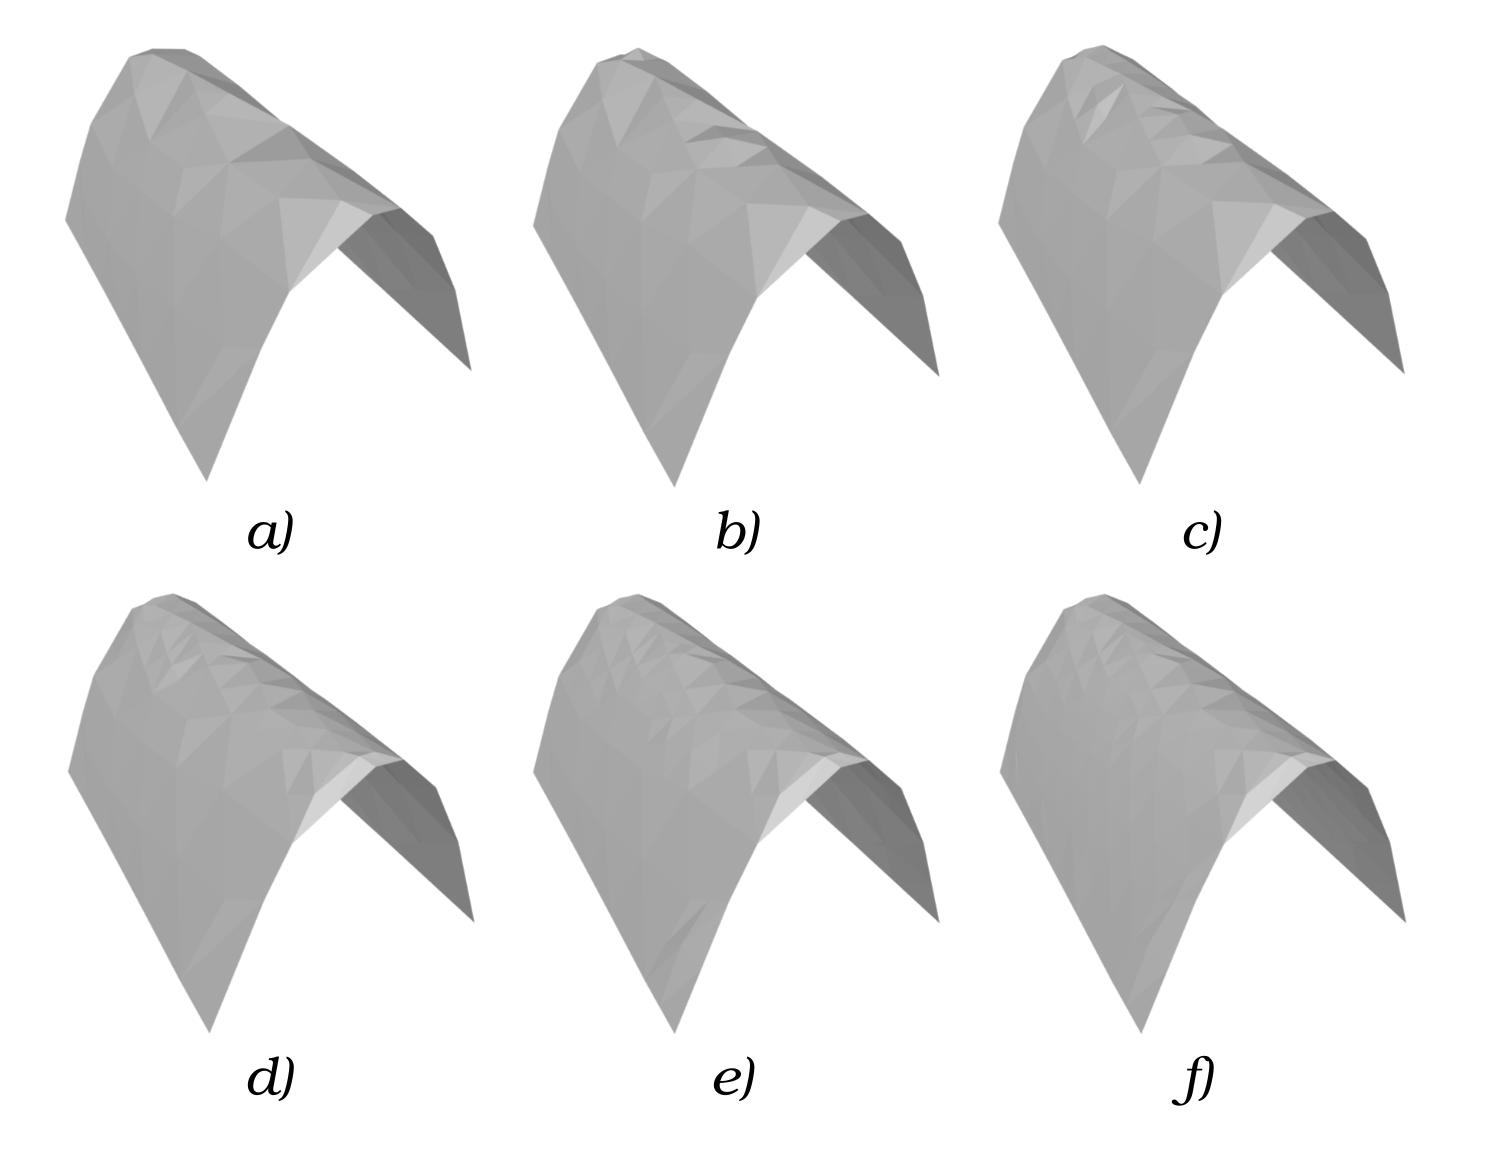
\includegraphics[width=0.6\textwidth]{images/adaptive_parabolic_cylinder}}
    \caption[Adaptívne prerozdelenie parabolického cylindra.]
    {$a)$ bez adaptívneho prerozdelenia, $b)$ $d=0.15$, $c)$ $d=0.1$, $d)$ $d=0.05$, $e)$ $d=0.03$, $f)$ $d=0.01$}
    %id obrazku, pomocou ktoreho sa budeme na obrazok odvolavat
    \label{obr:adaptive_parabolic_cylinder}
\end{figure}

\subsection{Prispôsobenie výšky nového trojuholníka}
Druhú metódu pre adaptívnu trianguláciu a to prispôsobenie výšky $k$ pri tvorbe nového trojuholníka 
vizualizujeme na niekoľkých modeloch.

Na modeloch pozorujeme, že pre vhodne zvolenú prahovú hodnotu $d$ nastáva prerozdeľovanie 
trojuholníkov v oblastiach s vyšším zakrivením, pričom trojuholníky v oblastiach s vyšším zakrivením 
zostávajú zachované.

Na obrázku \ref{obr:adaptive_height_ellipsoid} vidíme trianguláciu elipsoidu so zvolenou
dĺžkou hrany $a=0.9$.
\begin{enumerate}[a)]
\item{
    Základný neadaptívny algoritmus, výška trojuholníka volená ako výška rovnostranného trojuholníka
    s dĺžkou hrany $a$, teda $h=\frac{\sqrt{3}}{2} a$.
}
\item{
    Výška nového trojuholníka volená na základe aktuálnej hrany. Označme jej dĺžku e, potom  
    $h=\frac{\sqrt{3}}{2} e$.
}
\item{
    Výška nového trojuholníka volená na základe priemernej dĺžky aktuálnej hrany a jej susedných hrán. 
    Označme dĺžky susedných strán $e_{prev}$ a $e_{next}$, potom  
    $h=\frac{\sqrt{3}}{2} \cdot \frac{e+e_{prev}+e_{next}}{3}$.
}
\item{
    Výška nového trojuholníka volená na základe priemernej dĺžky aktuálnej hrany a jej susedných hrán
    pričom zohľadňujeme vplyv zvolenej dĺžky hrany $a$. Teda
    $h=0.75(\frac{\sqrt{3}}{2} \cdot \frac{e+e_{prev}+e_{next}}{3}) + 0.25 a$.
}
\end{enumerate}


\begin{figure}
    \centerline{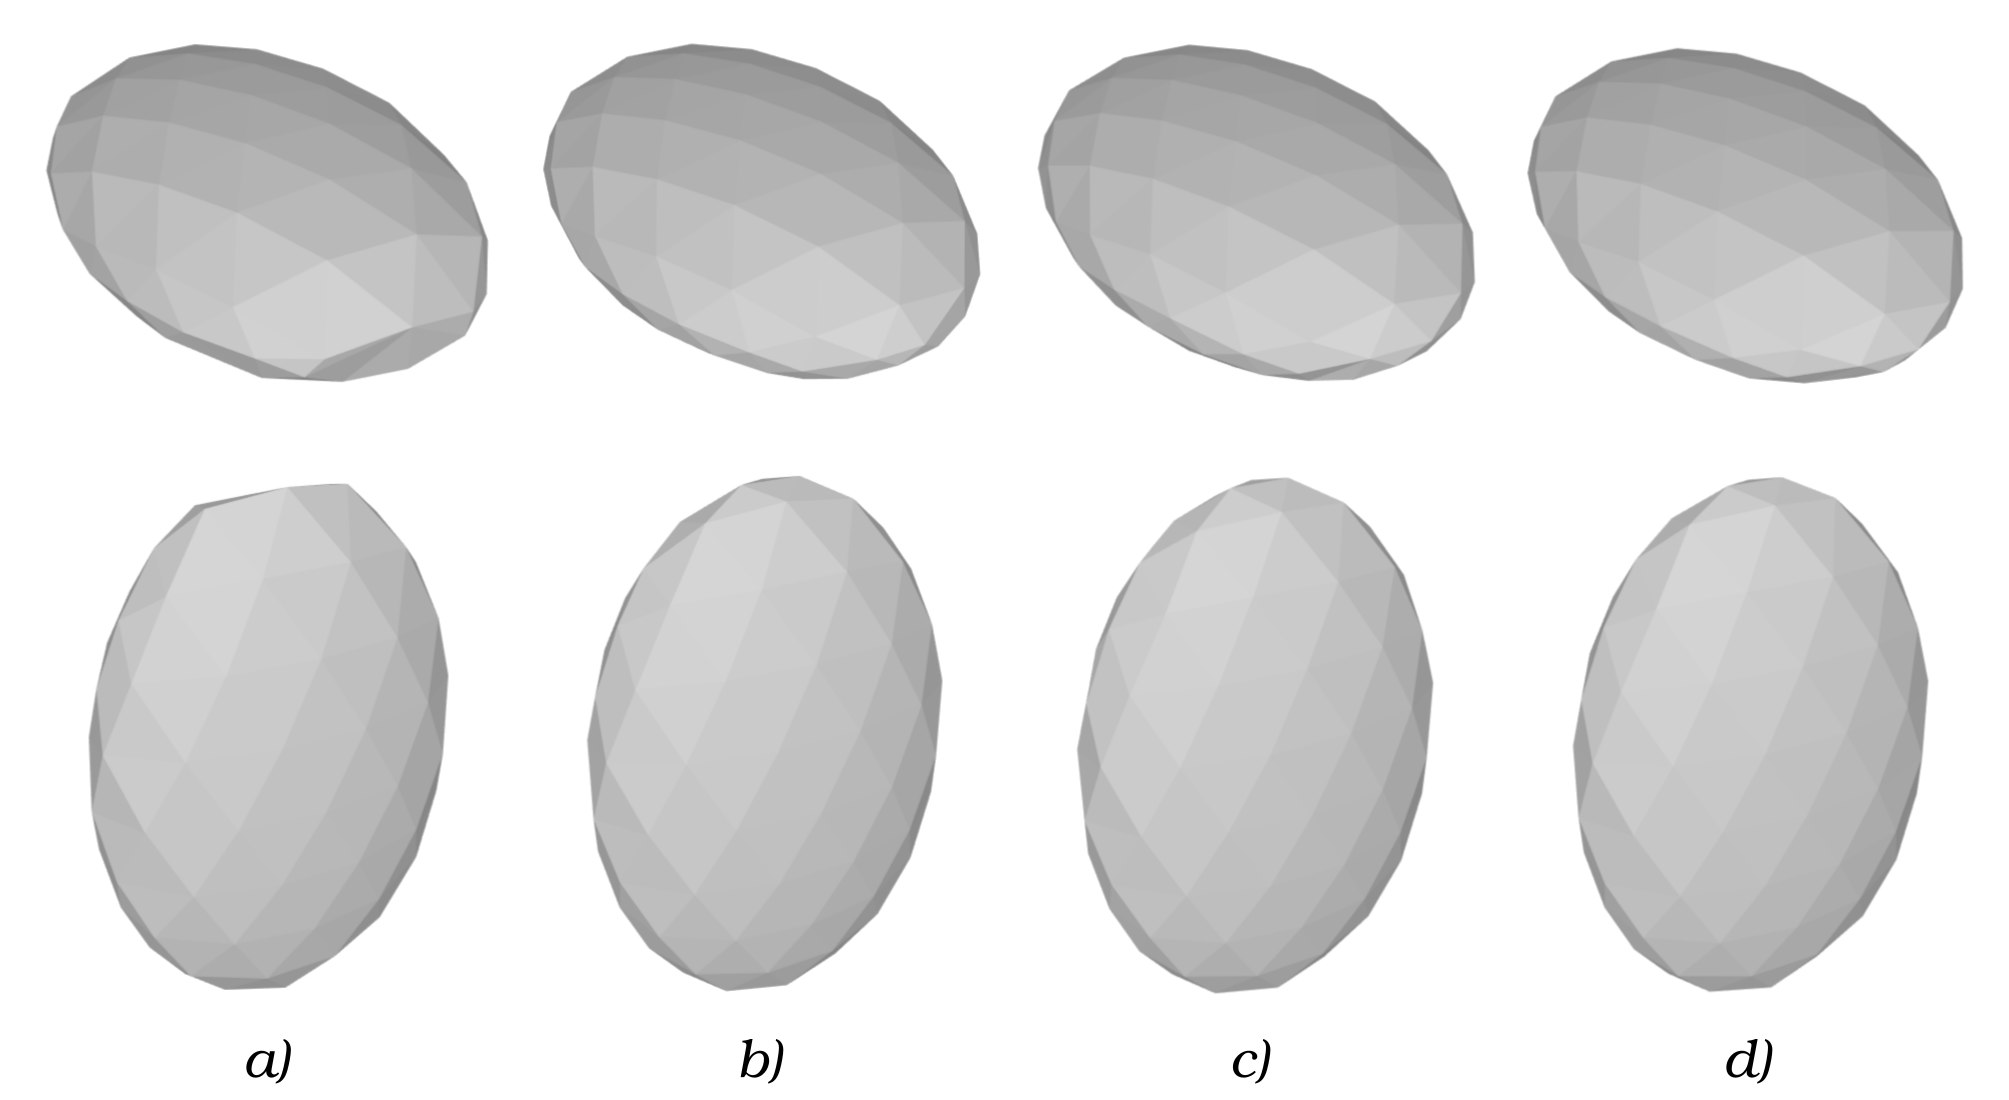
\includegraphics[width=0.8\textwidth]{images/adaptive_height_ellipsoid}}
    \caption[Adaptívna triangulácia elipsoidu]
    {Adaptívna triangulácia elipsoidu.}
    %id obrazku, pomocou ktoreho sa budeme na obrazok odvolavat
    \label{obr:adaptive_height_ellipsoid}
\end{figure}

Na obrázku \ref{obr:adaptive_height_tetrahedron} vidíme trianguláciu tetrahedronu so zvolenou
dĺžkou hrany $a=0.5$. Výšku nového trojuholníka volíme rovnako ako pri modeli elipsoidu.

\begin{figure}
    \centerline{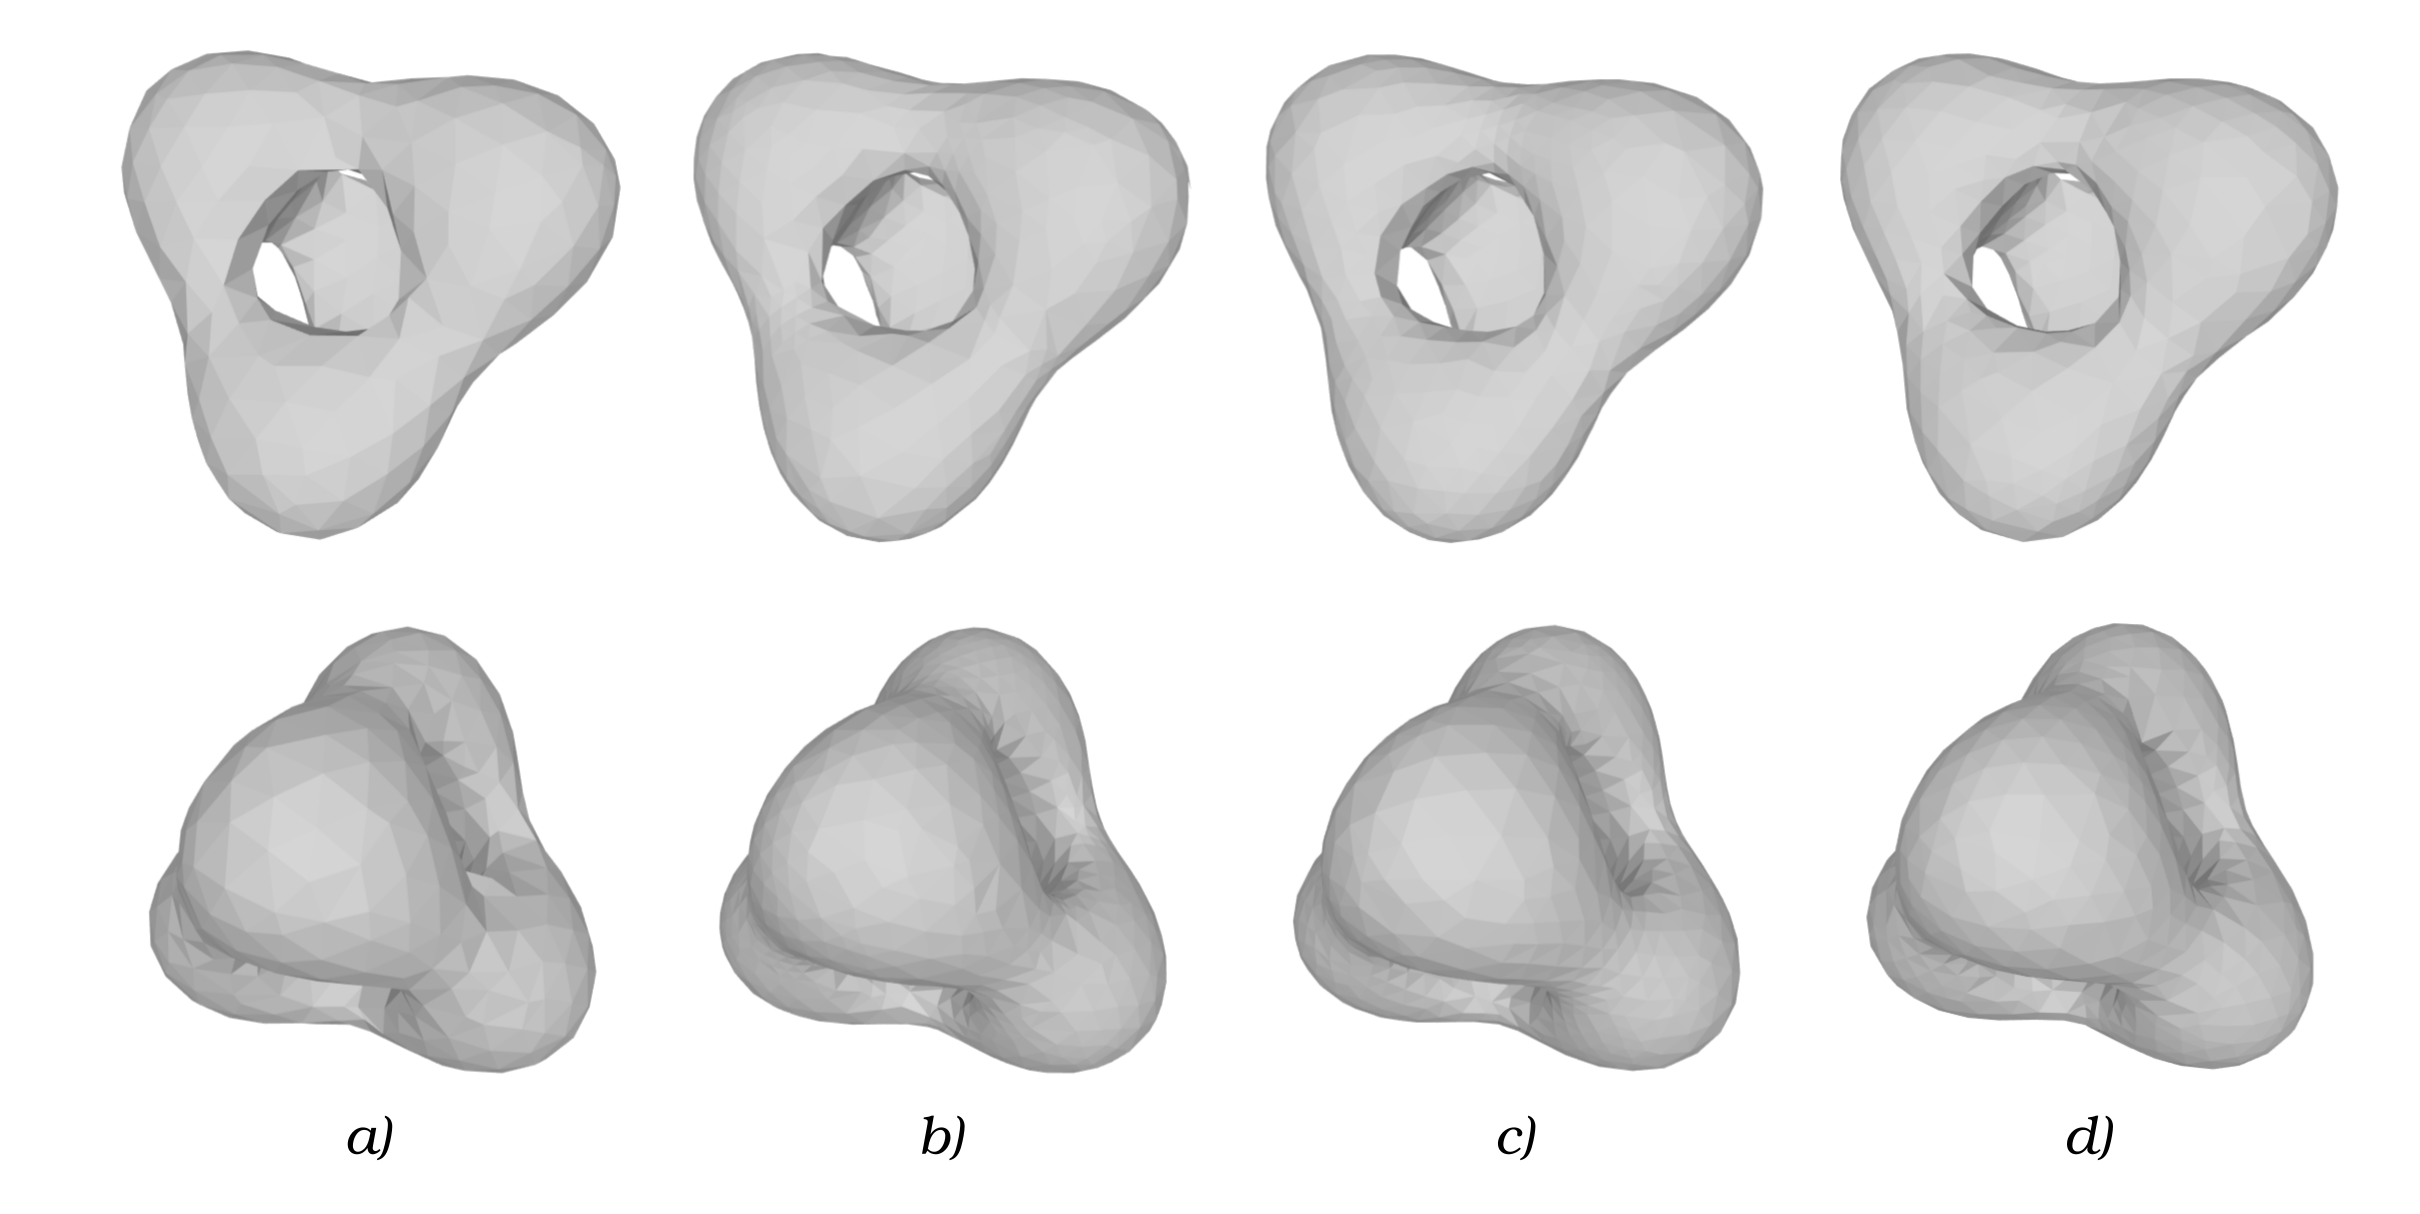
\includegraphics[width=0.9\textwidth]{images/adaptive_height_tetrahedron}}
    \caption[Adaptívna triangulácia tetrahedronu]
    {Adaptívna triangulácia tetrahedronu.}
    %id obrazku, pomocou ktoreho sa budeme na obrazok odvolavat
    \label{obr:adaptive_height_tetrahedron}
\end{figure}


\renewcommand{\arraystretch}{1}
\setlength{\fboxsep}{2mm} % box size
\setlength{\tabcolsep}{4pt}

    Nevýhoda, ktorú sme pozorovali pri výške založenej na aktuálnej hrane je občasné prekrývanie
    trojuholníkov, keďže \textit{Delaunayova podmienka} ani podmienka na zistenie blízkosti
    ťažiska nefungujú ideálne ak sa v triangulácii stretnú malý a veľký trojuholník.
    Ďalšou nevýhodou je veľké množstvo vznikajúcich trojuholníkov, keďže menšia hrana podmieňuje
    vznik menšieho trojuholníka a tento vplyv sa tak šíri ďalej.

    Pri prispôsobení výšky nového trojuholníka priemeru dĺžky aktuálnej hrany a dĺžok susedných 
    hrán pozorujeme už spomínanú nevýhodu. Trojuholníky zostávajú malé aj napriek tomu, že 
    sa už nenachádzajú v časti plochy s vyšším zakrivením a vytvára zbytočne veľké množstvo trojuholníkov.

    Tretí prístup eliminuje nevýhody oboch predchádzajúcich prístupov. Priemerovaním dĺžok hrán sa väčšinou 
    vyhneme stretnutiu veľmi malého a veľmi veľkého trojuholníka. Vplyvom zadanej dĺžky hrany pre 
    regióny s menším zakrivením trojuholníky opäť zväčšujeme a nevytvárame tak veľké množstvo zbytočných 
    trojuholníkov.

    Počty trojuholníkov jednotlivých triangulácii môžeme pozorvať v tabuľke \ref{tab:adaptive_height}.

    
\begin{table}[ht]
    \label{tab:adaptive_height}
    \caption[Porovnanie počtu trojuholníkov pre rôzne druhy adaptívnej triangulácie]{Porovnanie počtu trojuholníkov}
        \begin{center}
            \begin{tabular}{|c|c|c|c|c|}
                \hline
                \hline
                    & $a)$ & $b)$ & $c)$ & $d)$ \\
                \hline
                \hline
                $\hspace{3mm} Elipsoid \hspace{3mm}$ & $214$ & $300$ & $304$ & $266$ \EndTableHeader\\
                \hline
                $\hspace{3mm} Tetrahedron \hspace{3mm}$ & $1562$ & $2416$ & $2234$ & $1880$ \EndTableHeader\\
                \hline
                \hline
            \end{tabular}
        \end{center}
    \end{table}


    %The min, mid and max values
    %\renewcommand{\MinNumberA}{0.2}%
    %\renewcommand{\MidNumberA}{0.6} %
    %\renewcommand{\MaxNumberA}{1.0}%